
\documentclass[12pt,twoside]{article}
%%%%%%%%%%%%%%%%%%%%%%%%%%%%%%%%%%%%%%%%%%%%%%%%%%%%%%%%%%%%%%%%%%%%%%%%%%%%%%%%%%%%%%%%%%%%%%%%%%%%%%%%%%%%%%%%%%%%%%%%%%%%
\usepackage{amsfonts}
\usepackage{amssymb}
\usepackage{graphicx}
\usepackage{amsmath}
\usepackage[usenames,dvipsnames]{color}
\usepackage{tikz}
\usepackage{fancyhdr}
\usepackage{float}

\pagestyle{fancy}
\fancyfoot[l]{ECON0127}
\fancyfoot[re]{CONTINUED}
\fancyfoot[ro]{TURN OVER}
\fancyfoot[c]{\thepage}
\renewcommand{\headrulewidth}{0pt}

\textwidth15cm
\oddsidemargin1cm
\evensidemargin1cm
\topmargin0cm
\textheight20cm

\renewcommand{\u}{\upsilon}
\newcommand{\bF}{\mathbf{f}}
\newcommand{\bg}{\mathbf{g}}
\newcommand{\bp}{\mathbf{p}}
\newcommand{\bz}{\mathbf{z}}
\renewcommand{\bg}{\mathbf{g}}
\newcommand{\bw}{\boldsymbol\omega}
\newcommand{\bq}{\mathbf{q}}
\newcommand{\br}{\mathbf{r}}
\newcommand{\bQ}{\mathbf{Q}}
\newcommand{\bP}{\mathbf{P}}
\newcommand{\rd}{\;\mathrm{d}}
\newcommand{\re}{\;\mathrm{e}}
\newcommand{\rst}{\qquad\mathrm{s.t.}\qquad}
\def \vu {\overline{v}}
\def \vl {\underline{v}}
\def \wu {\overline{w}}
\def \wl {\underline{w}}
\renewcommand{\familydefault}{\sfdefault}

%\newcommand{\answer}[1]{\textbf{Answer:} {#1} \hfill $\square$}
\newcommand{\answer}[1]{}

\begin{document}

\begin{center}

\textbf{\large Term 2 2022-23}

\medskip
\textbf{\large ONLINE EXAMINATION}

\medskip

\textbf{\large ECON0127: Statistical Learning for Public Policy}

\end{center}

\medskip

All work must be submitted anonymously.  Please ensure that you add your \textbf{candidate number} and the module code to the template answer sheet provided. Note that the candidate number is a combination of four letters plus a number, e.g. ABCD9. You can find your candidate number in your PORTICO account, under “My Studies” then the “Examinations” container. Please, note that the candidate number is NOT the same as your student number (8 digits), which is printed on your UCL ID card. Submitting with your student number will delay marking and when your results might be available. 

\emph{Answer \textbf{ALL} questions from final.Rmd.  All questions carry equal marks.}

\textbf{Allow enough time to submit your work.} You are given 4 hours to solve your exam and an additional hour to submit your solutions on Moodle. This means that your work should be uploaded on Moodle \textbf{no later than 5 hours from the moment you accessed the examination paper for the first time}.

\emph{By submitting this assessment, \textbf{you pledge your honour} that you have not violated UCL’s Assessment Regulations which are detailed in 
\begin{center}
https://www.ucl.ac.uk/academic-
manual/chapters/chapter-6-student-casework-framework/section-9-student-academic-misconduct-procedure
\end{center}
which include (but are not limited to) plagiarism, self-plagiarism, unauthorised collaboration between students, sharing my assessment with another student or third party, access another student’s assessment, falsification, contract cheating, and falsification of extenuating circumstances.}

\pagebreak
\begin{enumerate}

\item Question 1

\begin{enumerate}
	\item Subquestion 1a
	I think that almost all the variables are relevant to predict \textbf{income\_group}. Infact, even though there are governments taking active actions against pay gaps due to \textbf{race, sex,} or \textbf{native\_country}, I personally think that these variables still have a strong impact on \textbf{income\_group}.
	Moreover I think that \textbf{marital\_status} has an impact on the income because a married person may have some children and statistically this could be correlated with him being fully committed to the career (correlation, not causal effect).
	Also, I initally thought that  \textbf{capital-gain/loss} describe the trend over time and they may not be impacting the current situation, but probably if there is a gain, it means that they are running a business that may be profitable. So I checked the relation between \textbf{capital-gain/loss} and the \textbf{income\_group} through the boxplots \ref{fig:capital_gain} and \ref{fig:capital_loss}. Therefore, I decided to include both of them because they seem to have an impact, especially \textbf{capital-gain}.
	Furthermore, even though \textbf{native-country} and \textbf{race} may seem correlated, I think that there could be a bias towards \textbf{race} in the job market and hiring processes. I also think that there could be people who have \textbf{race}=\textit{White}, but who come from South Africa or other countries, and since they are traveling abroad to pursue a career path, this may show that they are more committed than others with the same \textbf{race} but different value of \textbf{native-country}.
	Finally, I think that \textbf{education-num} and \textbf{edu} are highly correlated and this may lead to multiple collinearity that makes the model less efficient because it increases its variance and it is more prone to overfitting, so I remove \textbf{education-num} regressor.
	\begin{figure}[H]\centering
		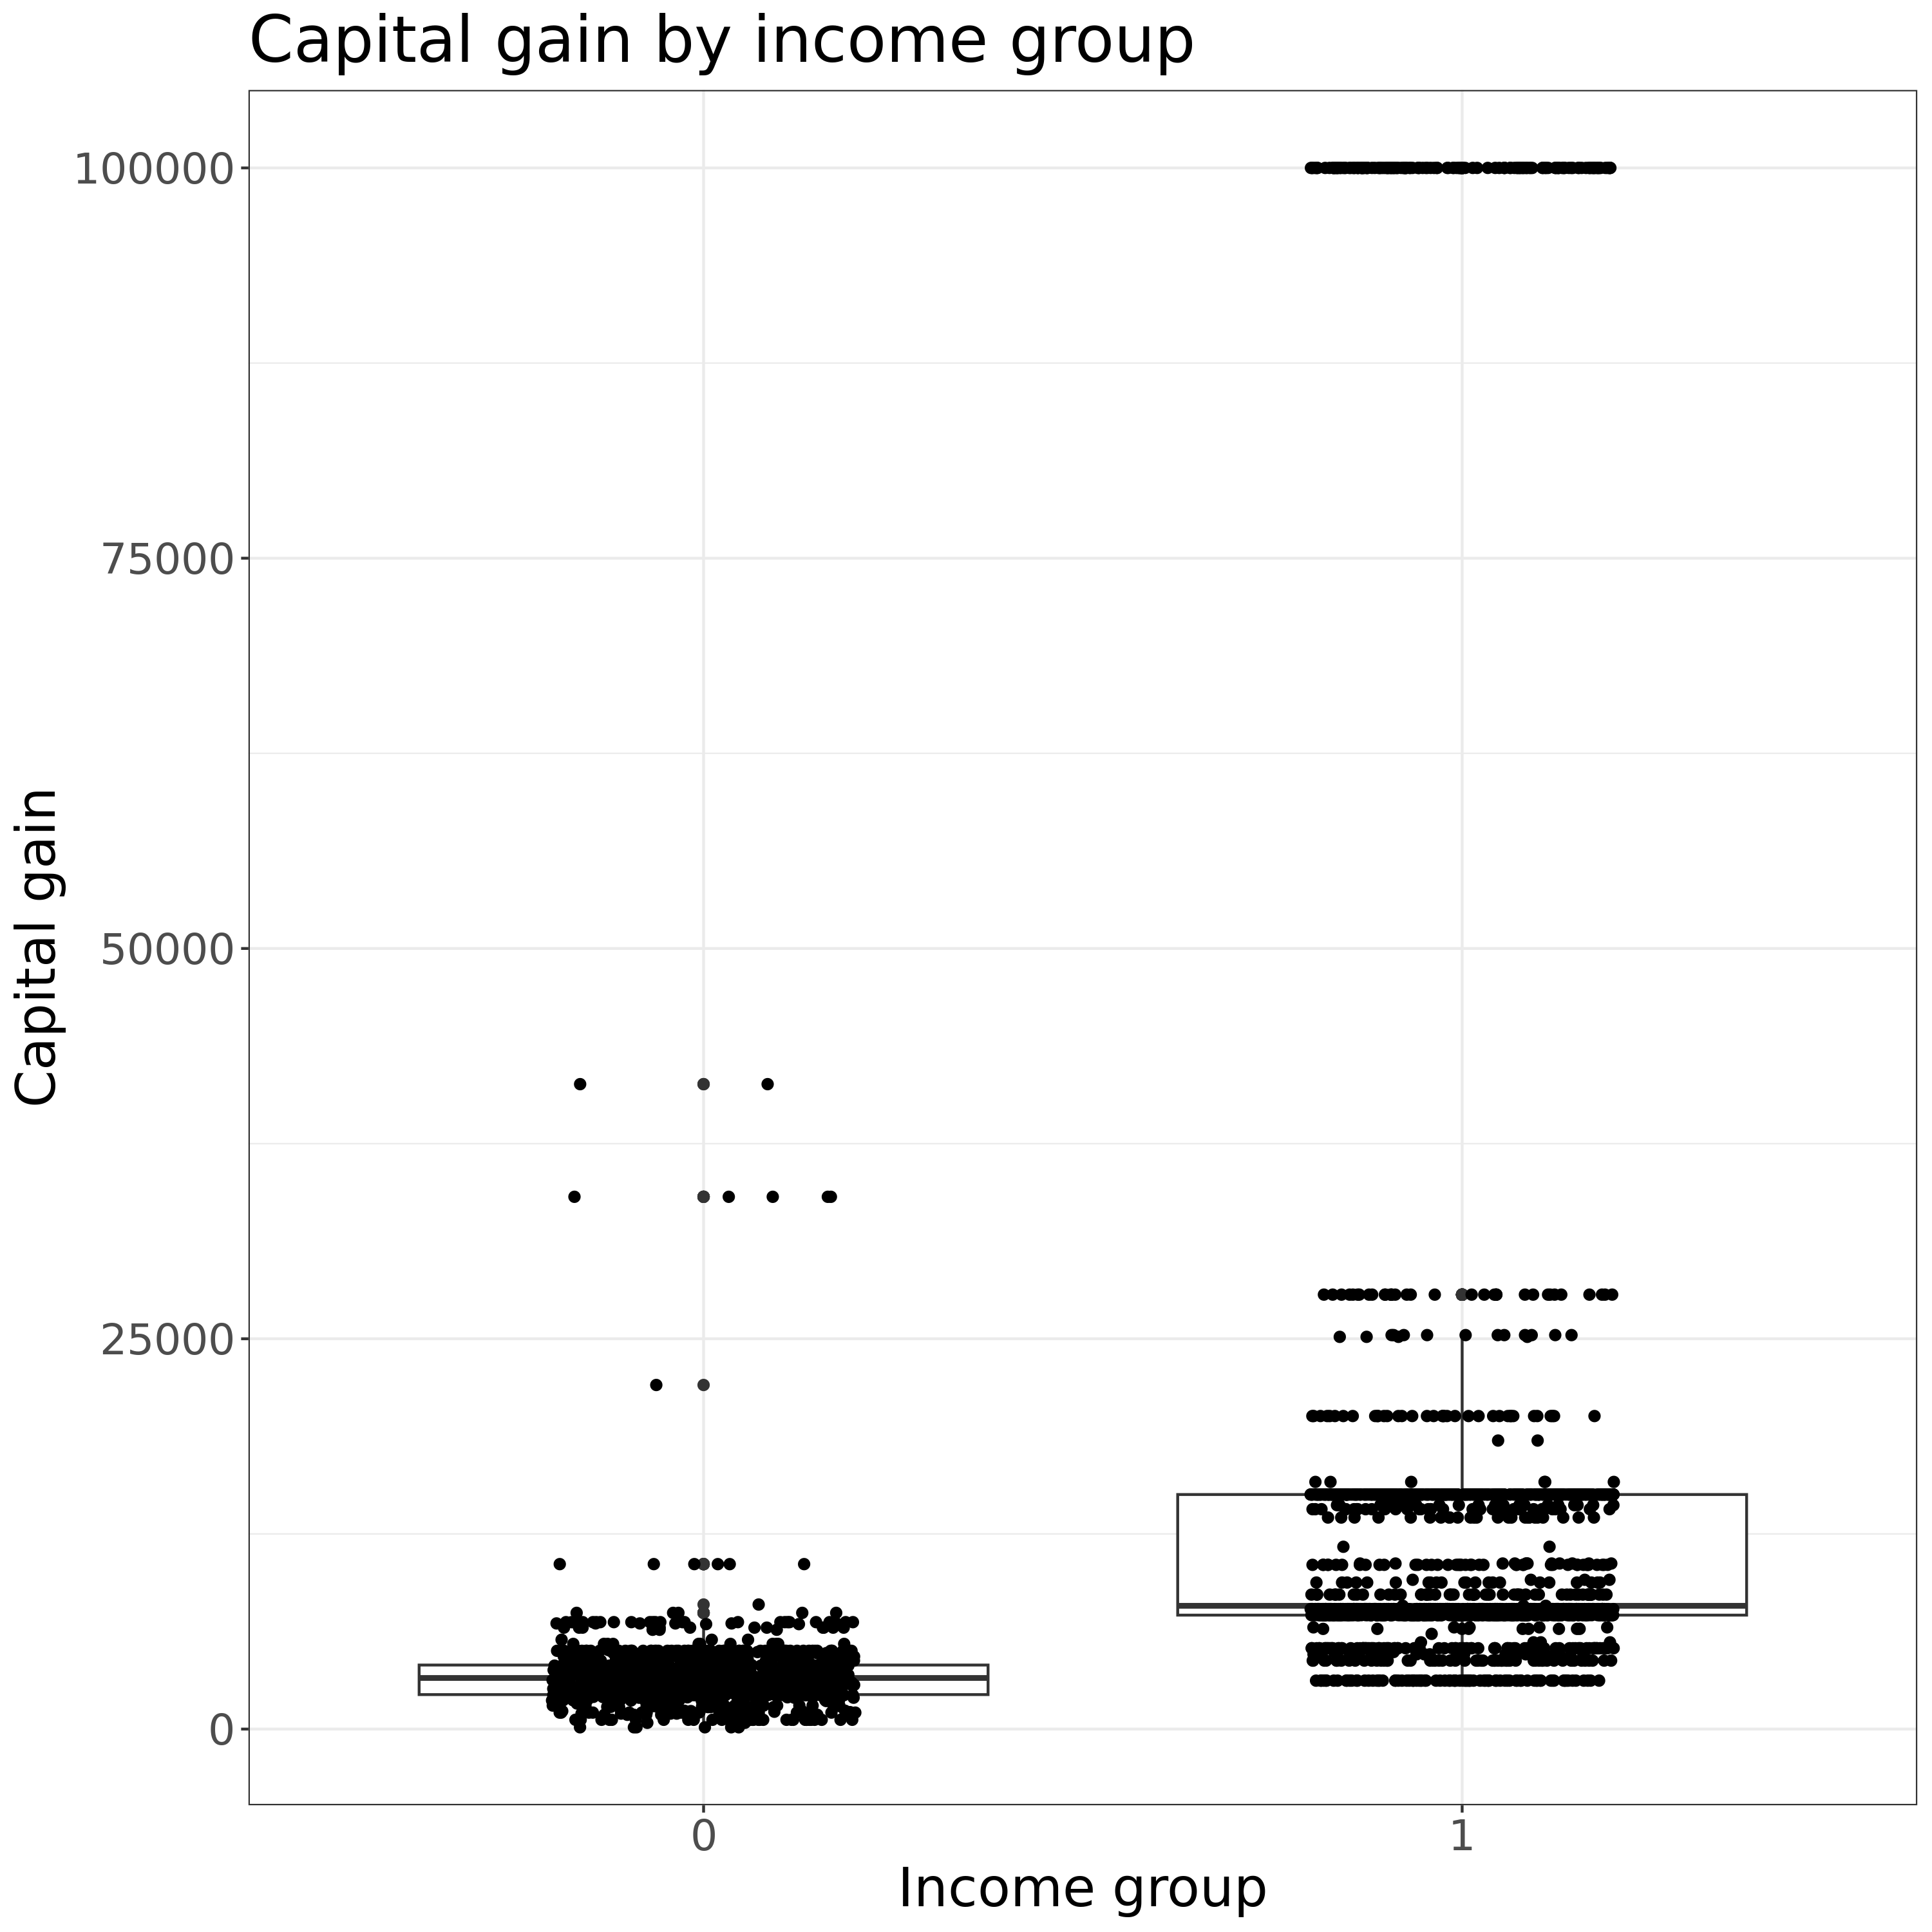
\includegraphics[width=8cm]{capital_gain}
		\caption{Boxplot used to check the \textbf{capital-gain} and the \textbf{income\_group}, where the samples with \texttt{capital-gain == 0} have been removed to improve readability.}
		\label{fig:capital_gain}
	\end{figure}
	\begin{figure}[H]\centering
		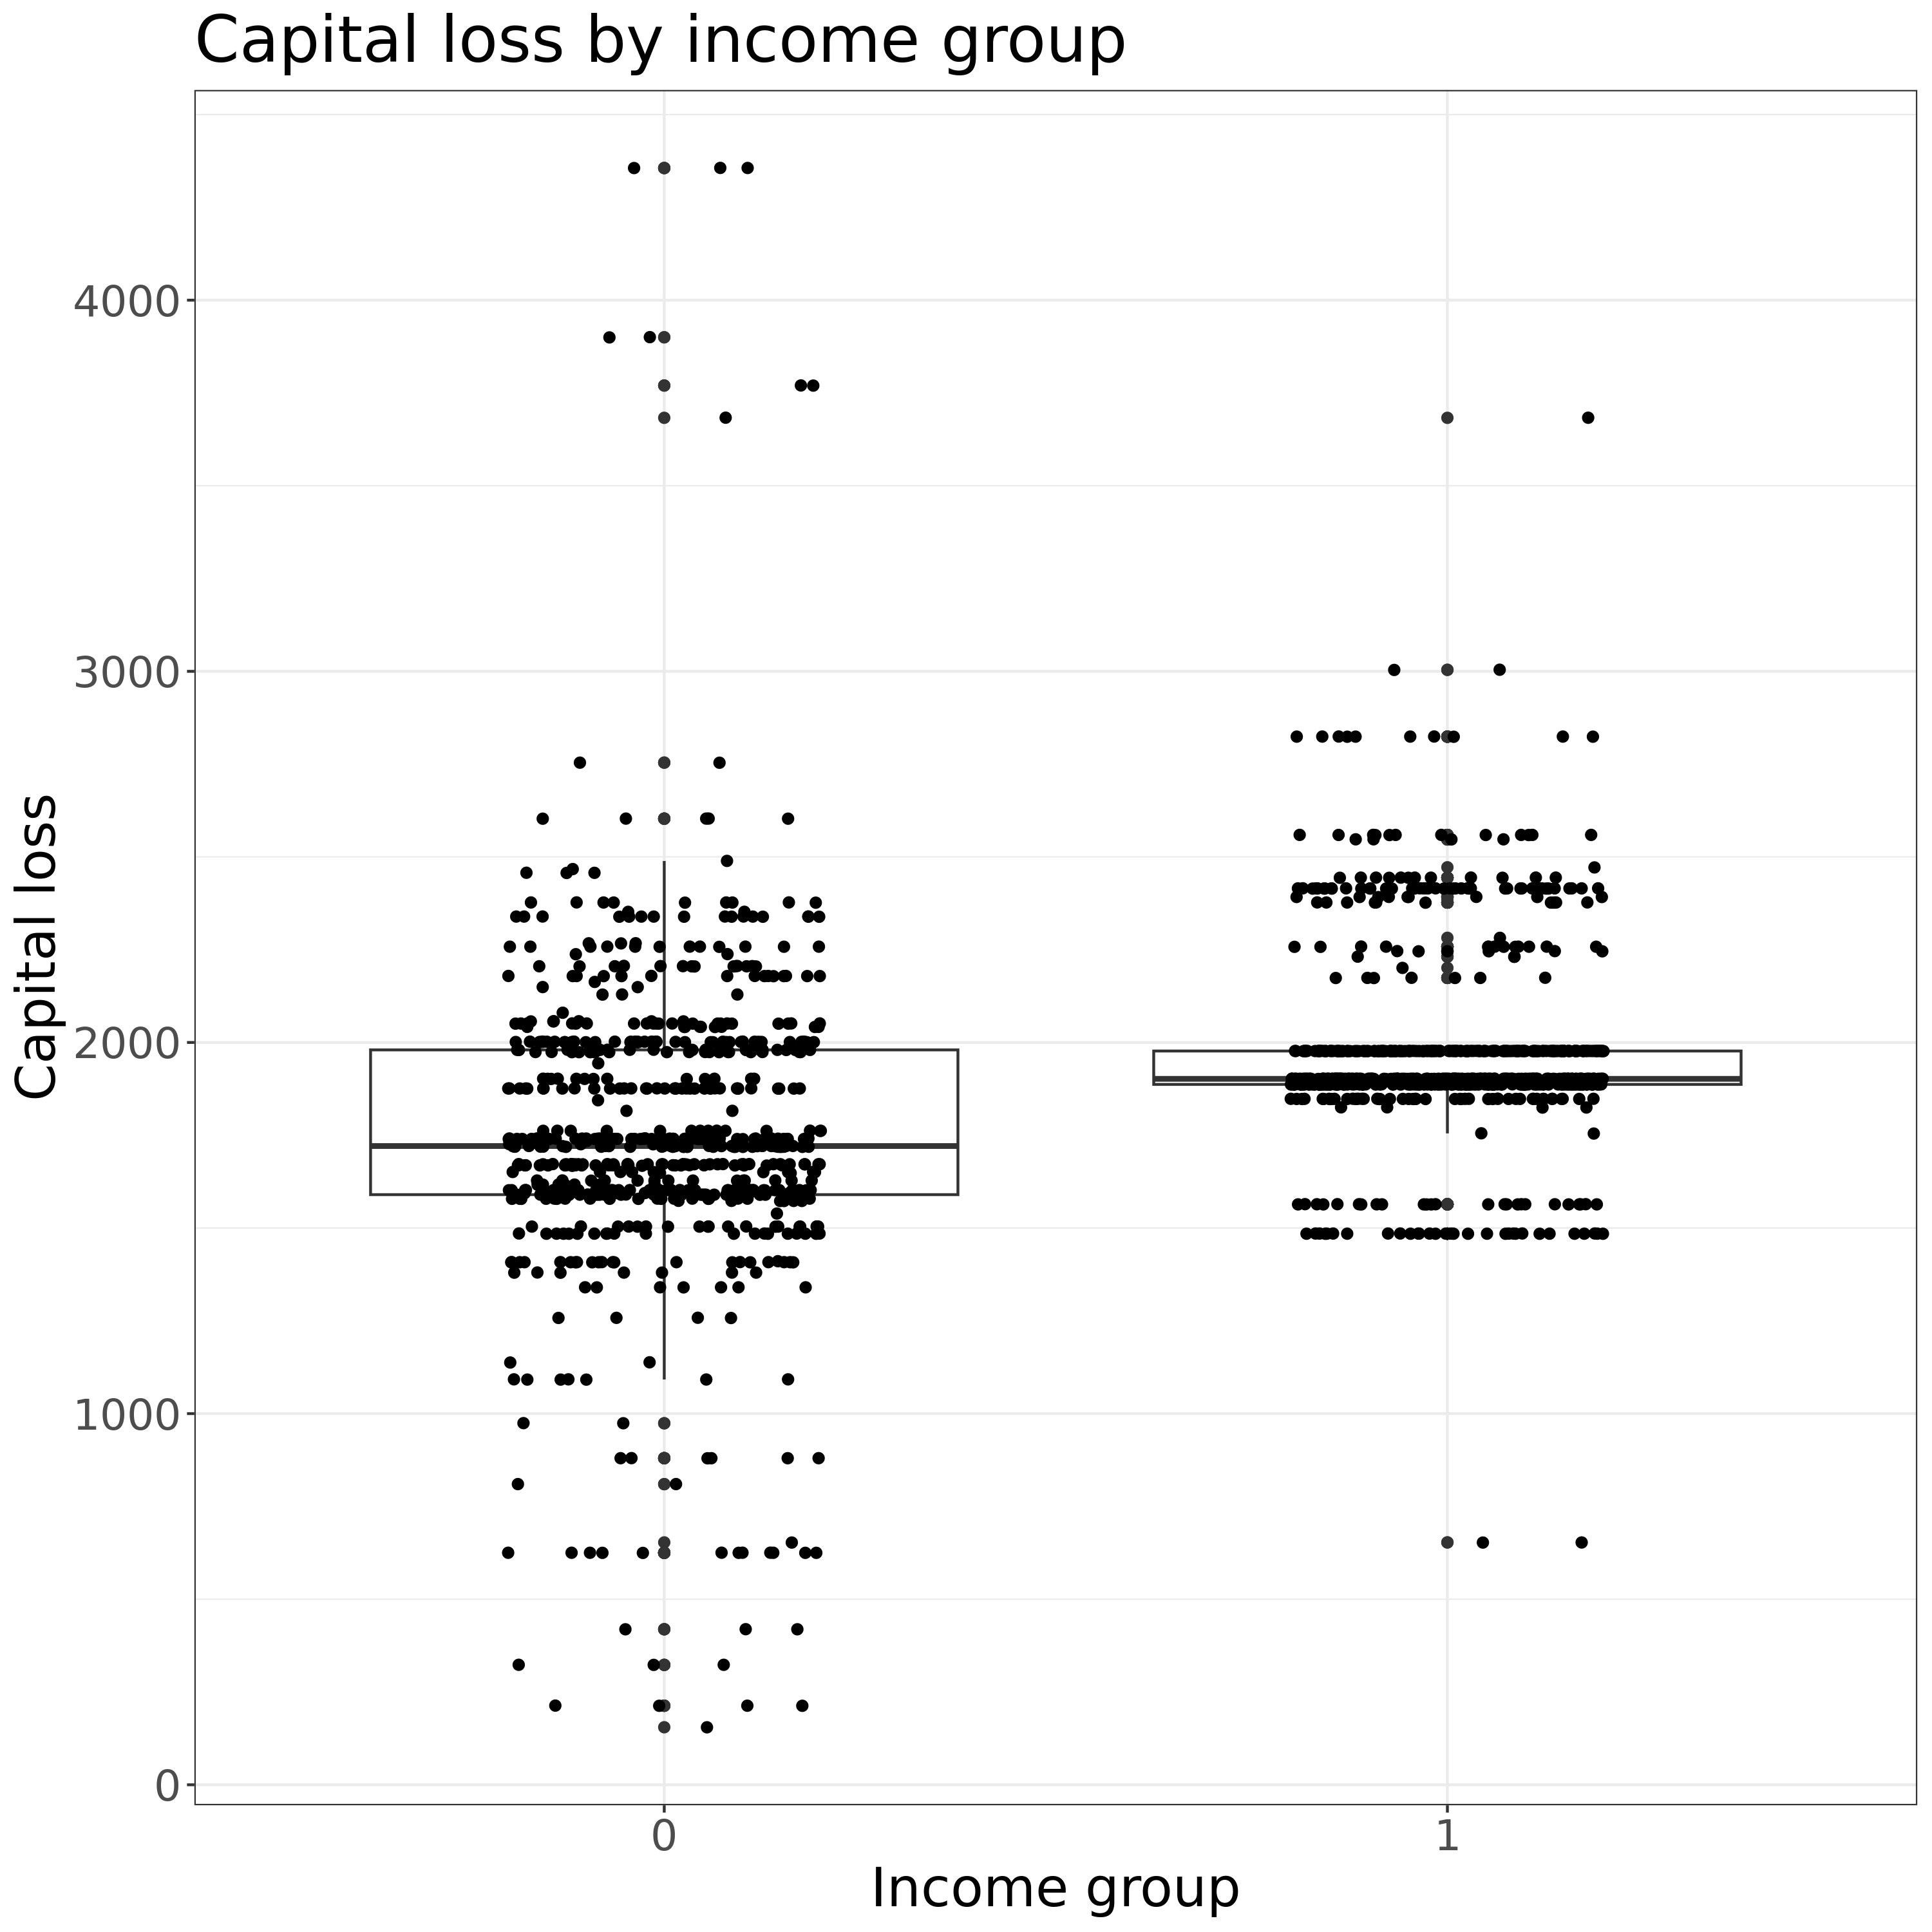
\includegraphics[width=8cm]{capital_loss}
		\caption{Boxplot used to check the \textbf{capital-loss} and the \textbf{income\_group}, where the samples with \texttt{capital-loss == 0} have been removed to improve readability.}
		\label{fig:capital_loss}
	\end{figure}
	\item Subquestion 1b 
	[Answer in the code]  For the data wrangling I was thinking of sorting the \textbf{education} covariate, since many of those values have a clear order. On the other hand, I would struggle with sorting the values of \textit{"Bachelors (university graduate)"} and \textit{"Some-college (some university)"} or the values \textit{"Prof-school (professional school)"}, \textit{"Assoc-acdm (associate degree - academic)"}, \textit{"Assoc-voc (associate degree - vocational)"}. So I will keep the covariate as type `factor` (transformed as One-Hot Encoded, or "dummy" variable). Moreover, in the dataset there are no NA values, so no rows are being removed.
	Since the \texttt{tree} package returns the error \texttt{"factor predictors must have at most 32 levels"}, I need to remove the rows that have the 10 least represented values of \textbf{native-country}, so I have to drop 143 rows out of 32561.
	\begin{figure}[ht]\centering
		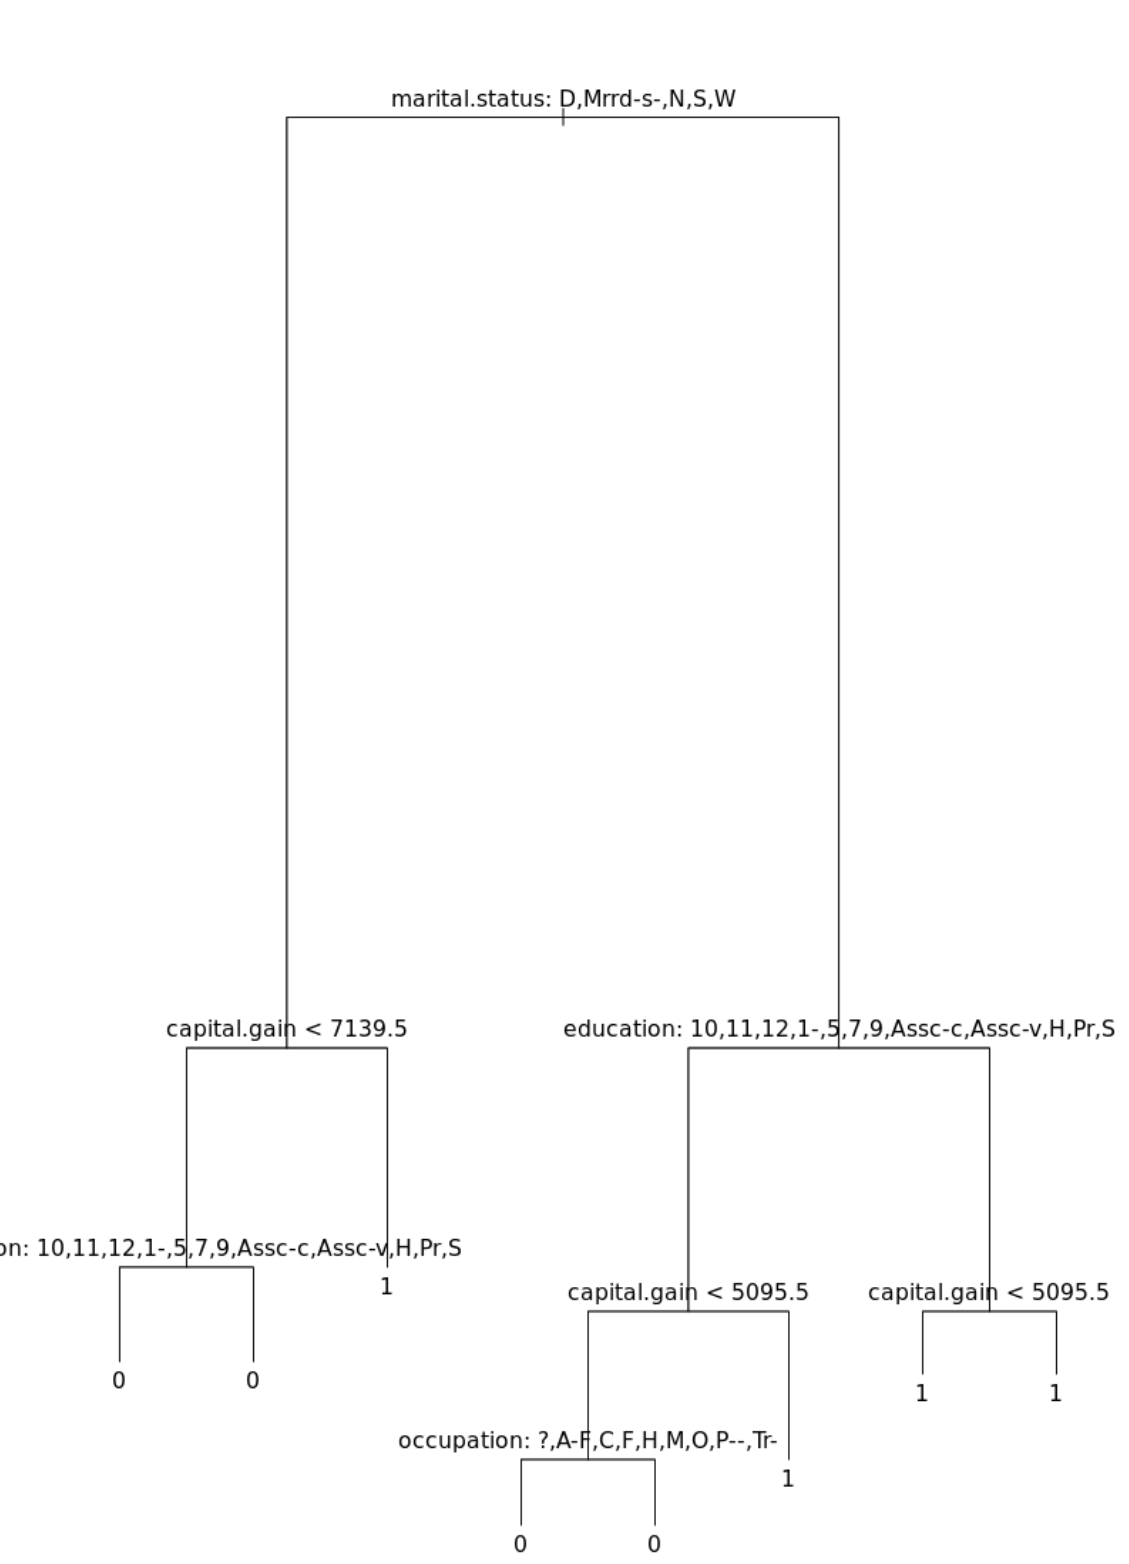
\includegraphics[width=12cm]{decision_tree}
		\caption{Decision tree trained on the whole dataset to predict \textbf{income\_group} outcome variable.}
		\label{fig:decision_tree}
	\end{figure}
	The tree has the structure shown in \ref{fig:decision_tree}. We can notice that initially the dataset is split based on its \textbf{marital.status} and if this is equal to \textit{Divorced, Never-married, Separated, Widowed or Married-spouse-absent} then we have to follow the left branch. In this case, if the capital-gain of the respondent is $< 7139.5$, then his/her income\_group is 0 (<50K per year), otherwise it is 1.
	Viceversa, if the \textbf{marital.status} is not one of those values listed above, then we can follow the right branch and see that if the respondent has not one of the listed \textbf{education} values, so it has either one of (\textit{Bachelors (university graduate), Masters (masters degree), Doctorate, }), it is more likely that he has an income >50K, independently of its \textbf{capital-gain}.
	In conclusion, we can say that it is more likely that a respondent has a yearly income higher than 50K if he/she has a married partner who is also working, and/or if he/she has an education degree equal to Bachelors degree or higher, like Master and Doctorate. In contrast to this, \textbf{sex} and \textbf{race} do not look relevant based on this decision tree. On the other hand, as we explain in Q1.c, decision trees are not very stable and they are very sensitive to small changes in data, especially when the variable are correlated to each other. For inference purposes, Causal Forest and Honest Forest are more advisable.
	
	I obtain \textit{Accuracy}$=0.8438$ and \textit{AUC}$=0.7315$ on the whole dataset (that was used for training the tree).  I also computed the Area Under the Curve (AUC) score, since it is a binary classification problem and the accuracy may not describe the model performance accurately, especially with highly imbalanced classes, like in this case with 24604 samples having 0 as \textbf{income\_group} and only 7814 having 1.
	Infact, if the model was trivial and only outputs 0 for every possible input, the accuracy on this dataset would still be $24604/(24604+7814)=0.7590$, but the AUC would be close to 0.5, which is as good as a random choice.
	
	\item Subquestion 1c First I set the seed to 123 for reproducibility, then I randomly split the dataset into train-test set with 80/20 ratio. The test-set accuracy of the decision tree is 0.8436 and its AUC score is 0.7296
	Due to the imbalanced classes, we could a performance improvement by splitting the dataset into train and test set in a stratified fashion, in order to have a similar ratio of the 2 classes both in train and test set.

	Decision trees are usually not considered a robust prediction algorithm because they have high variance, meanly they are prone to overfitting, especially when they are grown deep with many branches and leaves. This means that they can fit the training data too closely and perform poorly on unseen data. 
	For the same reason, the decision trees are very sensitive to small changes in the training data, so even a small modification may result in a completely different tree structure. Moreover, they struggle to capture complex patterns and relationships in the data, and to achieve good performances when the outcome is a continuous function of the regressors, because a single tree always creates discontinuous regions in the regressor space.
	
	\item Subquestion 1d 
	We might expect the bagging approach to produce better test-set performance than our previous decision tree because the bagging algorithm reduces the variance by averaging the predictions of many bootstrapped trees, also called \textit{forest}. Particularly bagging algorithm introduces some randomness into each decision tree by using only a bootstrap sample of the whole dataset to train each tree (every sample has the same number of observations, but some of them are missing, while others are repeated). So each tree is trained using slightly different data. 
	As we previously mentioned, decision trees are very sensitive to small changes in the training data, so every tree may turn out quite different from each other, but the average of their predictions can give a more stable result with less variance.
	
	Employing the bagging algorithm with 50 bootstrap samples (or replications), we get Accuracy$=0.8510$ and AUC$=0.7778$ which is higher than the decision tree (AUC=0.7296) from Q1.c
	
	\item Subquestion 1e 
	By increasing the number of trees, the bagging model can improve its performances in capturing complex relationships and patterns in the data, by becoming more flexible and adaptive. As more diverse trees are included, the ensemble decrease its variance, meanly its sensitivity to small changes in data. So, by combining predictions from more and more trees, the ensemble's aggregated predictions tend to smooth out individual tree errors, and the model is expected to increasingly reduce the risk of overfitting and improve regularization. This should lead to improved test-set performance, especially when individual trees are prone to overfitting due to their complexity or depth.

	In figure \ref{fig:accuracy_auc_per_num_trees} we can notice how accuracy and AUC score improve when the number of trees employed by the bagging algorithm increases, confirming our expectations.
	\begin{figure}[H]\centering
		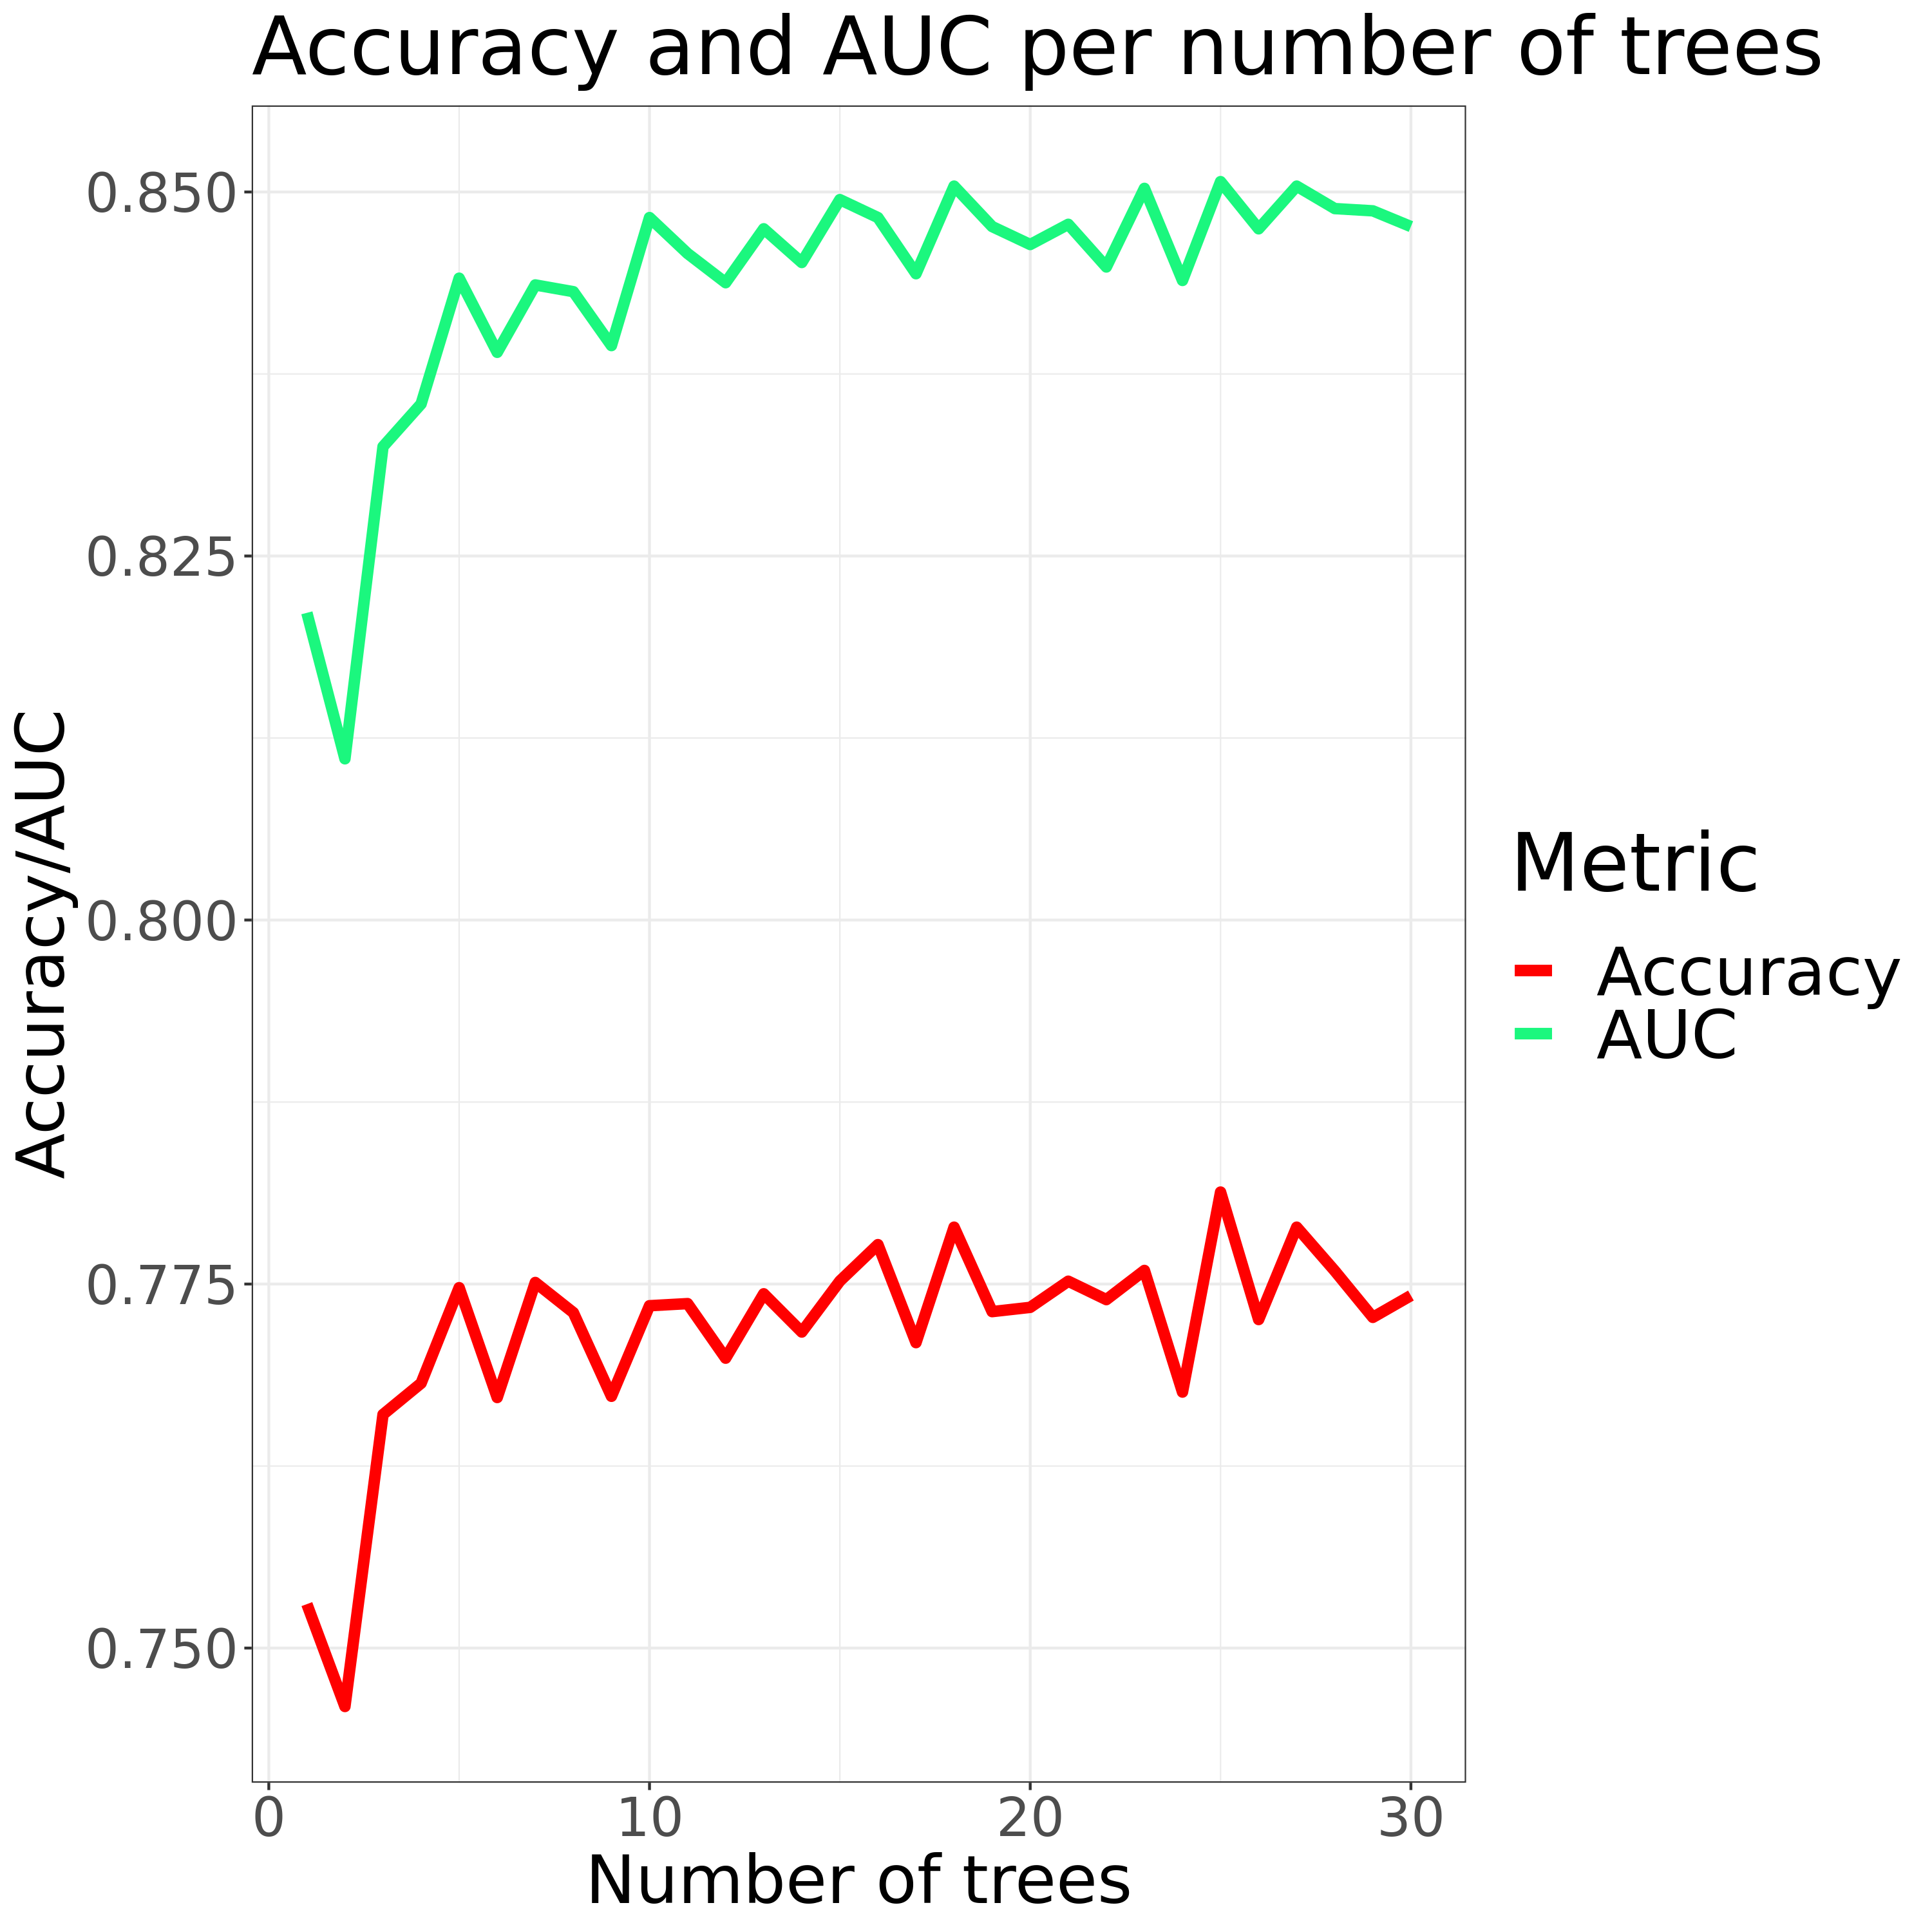
\includegraphics[width=12cm]{accuracy_auc_per_num_trees}
		\caption{Accuracy and AUC score per number of trees (and bootstrap replicates) used by the bagging algorithm.}
		\label{fig:accuracy_auc_per_num_trees}
	\end{figure}

\end{enumerate}

\item Question 2

\begin{enumerate}
	\item Subquestion 2a
	The neural network described is called a "\textit{single layer network}" where we have a scalar as input (\texttt{input\_shape = 1}) and a scalar as output (i.e. the outcome variable). In the middle we add a hidden layer with 5 nodes.
	More specifically in the input layer, in addition to the 1-dimensional input, a bias is automatically added, such that there are 1 node and the bias fully connected with each of the 5 nodes of the hidden layer with a certain weight $\theta_{j,k}$, so that there are 10 different weights, which are trainable parameters of the neural network.
	So each node k (k=1..5) of the hidden layer is the result of the linear combination of the bias "1", weighted with $\theta_{0,k}$ and the input parameter $x_{i}$ weighted with  $\theta_{1,k}$:
	\begin{equation}
		z_i=\theta_0+\theta_1 * x_{i, 1}
	\end{equation}
	Then on the result of the linear combination of each node we apply a non-linear function called "Rectified Linear Unit" (ReLu).
	Similarly the output layer is the result of the linear combination of the outputs of each of the 5 nodes in the hidden layer, plus the bias, where every element is weighted with a weight $\theta_{j,1}$, so that we have 5+1 weights, or trainable parameters:
	\begin{equation}
		y_i=\theta_{0,1}+\sum_{j=1}^5 \theta_{j,1}* ReLu(z_{i, j})
	\end{equation}
	So in total we have $$(1+1)*5 + (5+1)=16$$ trainable parameters in our network.
	\item Subquestion 2b 
	The first step in estimating a neural network is to define an objective function (called "loss function") to minimize. In this case, we use the Mean Squared Error:
	\begin{equation}
		L(\boldsymbol{\theta})=\frac{1}{N} \sum_{i=1}^N L^{\prime}\left(y_i, f\left(\mathbf{x}_{\mathbf{i}} \mid \boldsymbol{\theta}\right)\right)
	\end{equation}
	where:
	\begin{equation}
		L^{\prime}\left(y_i, f\left(\mathbf{x}_{\mathbf{i}} \mid \boldsymbol{\theta}\right)\right)=-(y_i - f\left(\mathbf{x}_{\mathbf{i}} \mid \boldsymbol{\theta}\right))^2
	\end{equation}
	Then we employ a \textit{gradient descent }algorithm that, at each step, tries to modify the weights in order to minimize the loss function:
	\begin{enumerate}
		\item Randomly initialize $\mathbf{theta}$
		\item For every sample of the dataset, compute the gradient and update the weights:
		\begin{equation}
			\boldsymbol{\theta}^i=\boldsymbol{\theta}^{i-1}-r \nabla L\left(\boldsymbol{\theta}^{i-1}\right)
		\end{equation}
		where r is the learning rate, meanly the speed at which we are gonna update the trainable parameters of the network in order to approach the local minimum of the loss function, so it is usually set to a small number.
	\end{enumerate}
	In this case, we are gonna use an optimizer for the learning rate called "Root Mean Square Propagation", which is an adaptive learning rate optimization method, commonly used in Neural Network, that adjusts the learning rate for each parameter based on the magnitude of recent gradients. Specifically, it gives more weight to recent gradients while dampening the influence of earlier gradients, so that the earlier gradients do not affect the learning rate much and it prevents the learning rate from becoming too large or too small based on them, because this may lead to convergence issues, like getting stuck in local minima or in flat areas of the loss function.
	Moreover, the code above specifies that we are gonna use a mini-batch stochastic gradient descent where data is initially randomly shuffled and then cycled through chunk by chunk (mini-batch) where each batch contains 50 samples. The batches are not overlapping. Once the algorithm has cycled through the whole dataset, this is called an \textit{epoch}.
	This whole algorithm gets repeated 1000 times/epochs in our case.

	\item Subquestion 2c 
	This neural network is unlikely to be able to approximate well the function because it contains only one output layer with one node so, assuming a one-dimensional input (with only 1 regressor), its output function is defined as:
	\begin{equation}
		y_i=sigmoid(\theta_{0}+\theta_1*x_i)
	\end{equation}
	So we are just applying a non-linear function to a linear combination of the regressor and the bias, so if the relation between the regressor and the outcome variable was defined by a polynomial, it would not be possible for this network to reproduce the same relation just by training the parameters/weights (figure \ref{fig:one_layer_preds}).
	According to Universal Approximation Theorem, infact, we need at least one hidden layer to be able to approximate any function.
	\begin{figure}[H]\centering
		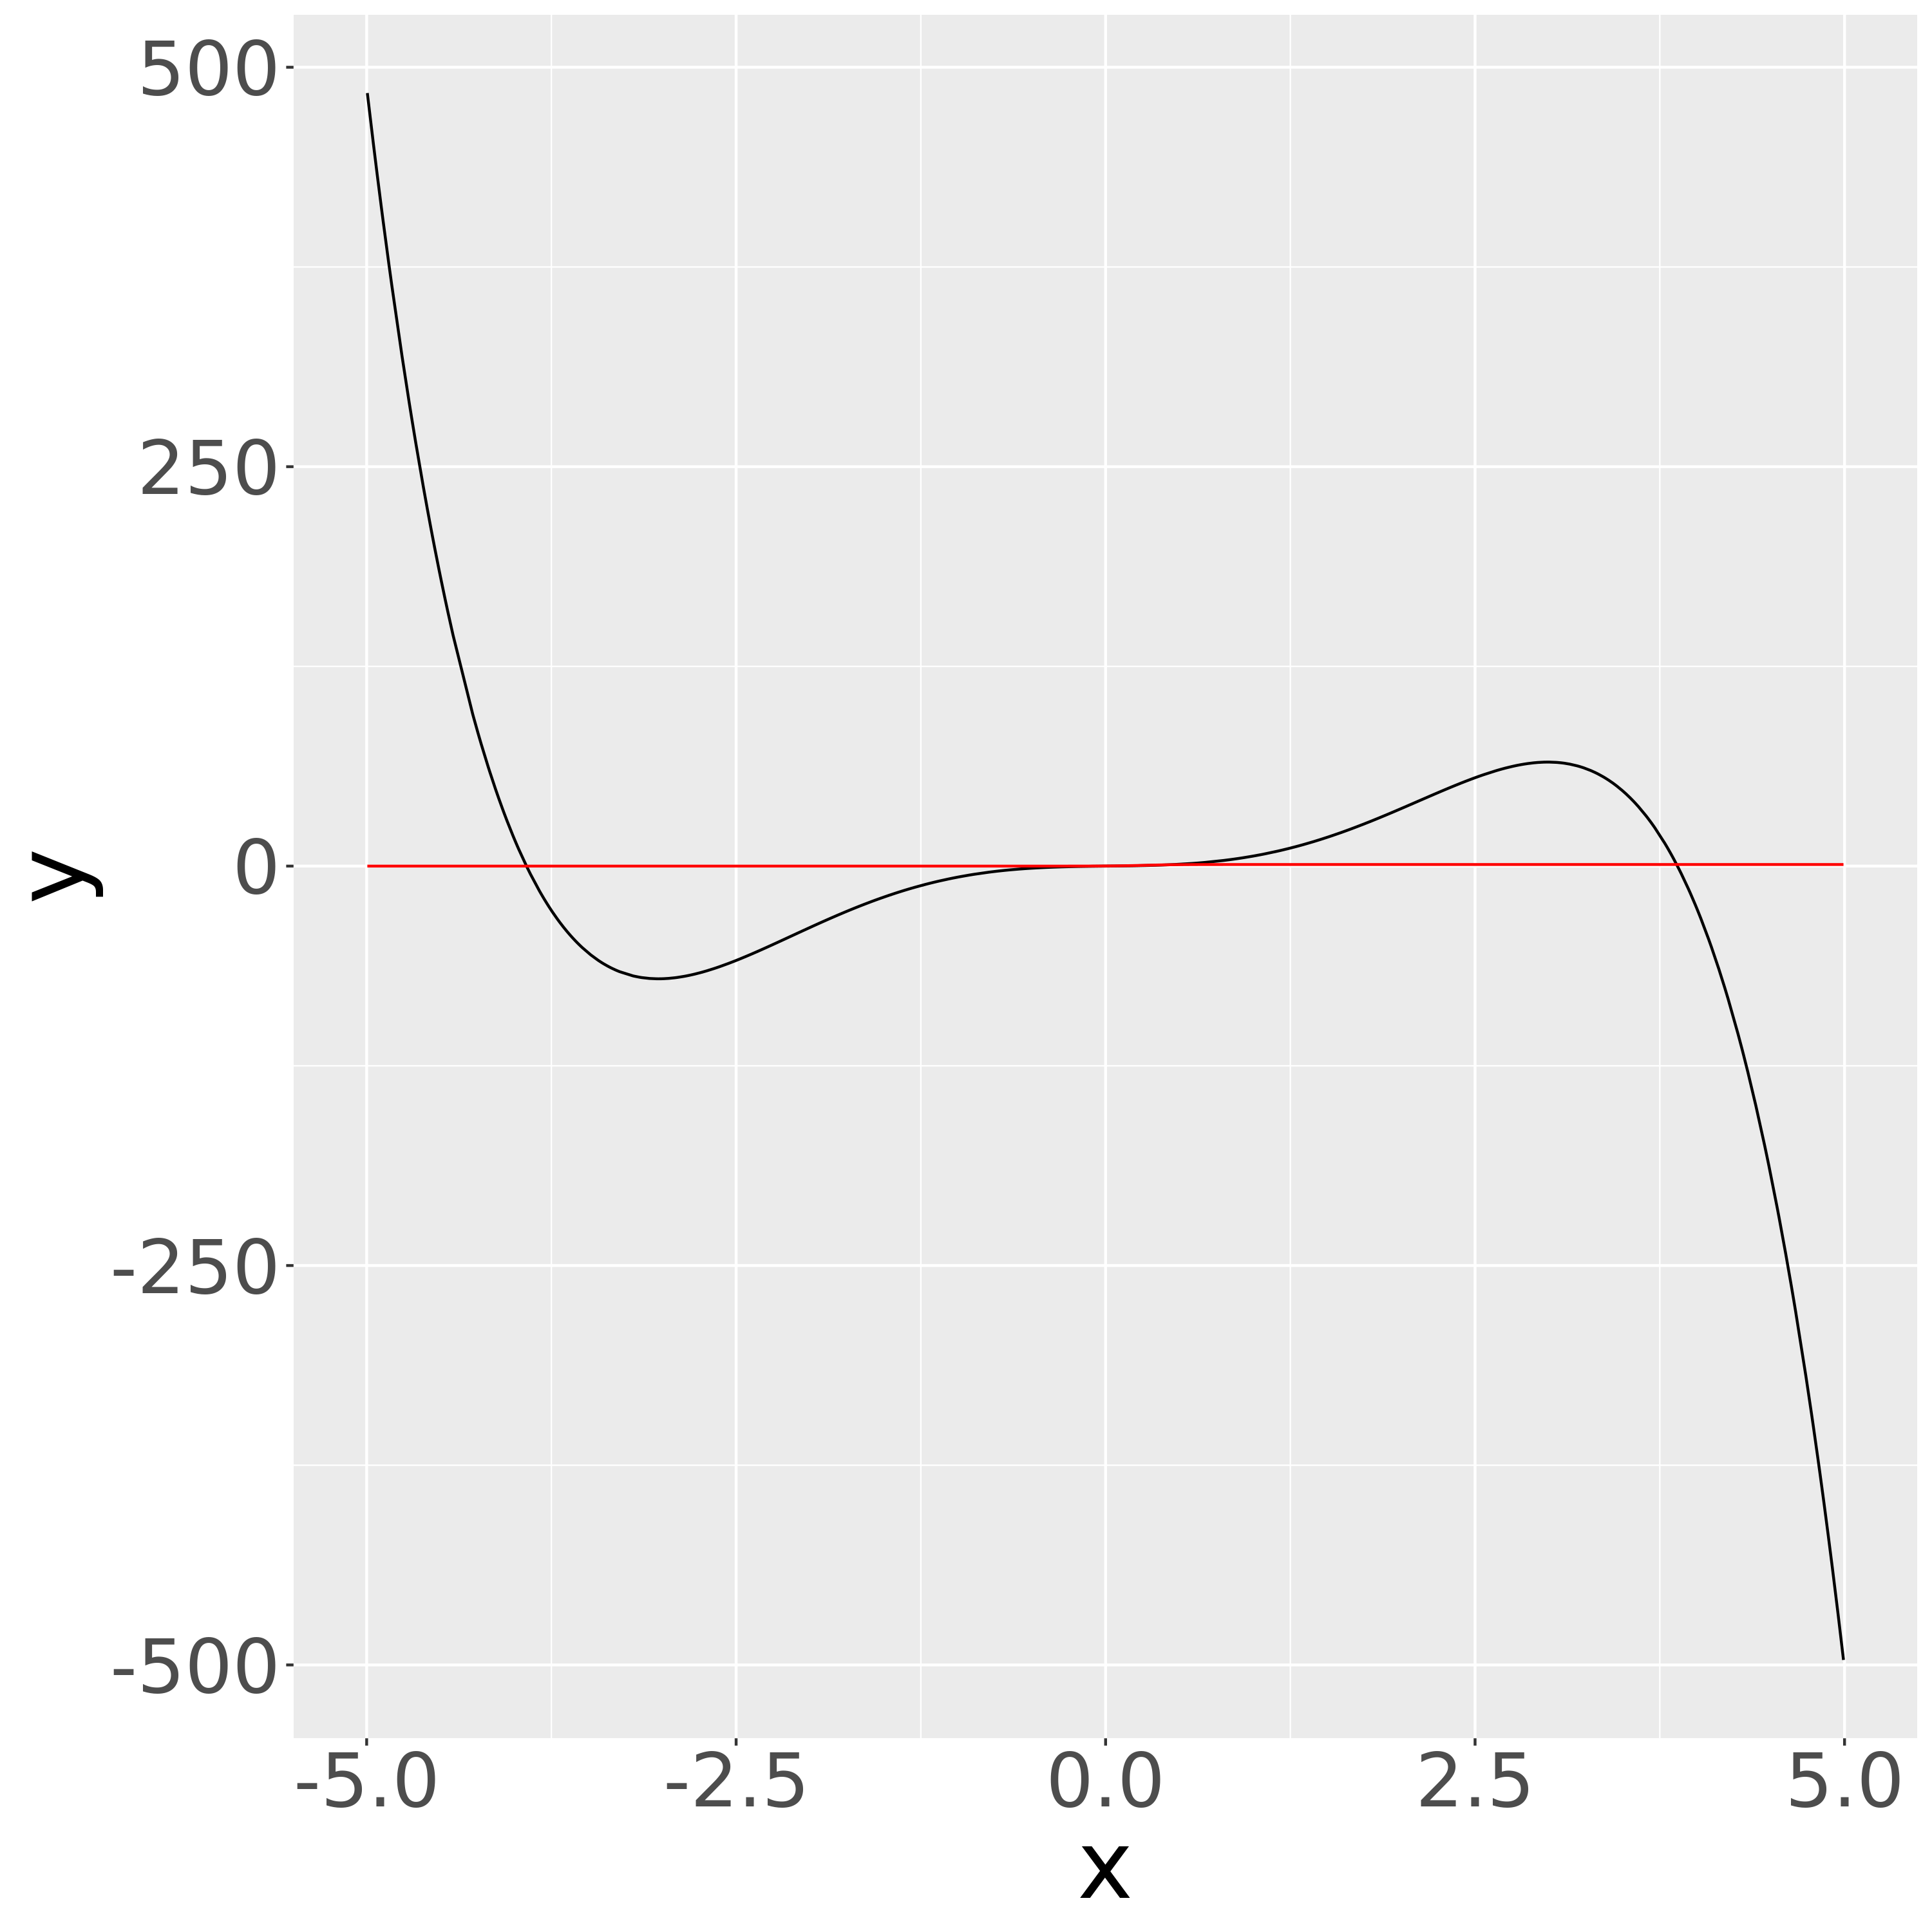
\includegraphics[width=7cm]{one_layer_preds}
		\caption{Comparison between the function fitted by the 1-layer Neural Network (red) from Question 2.c and the original function, or ground truth (black).}
		\label{fig:one_layer_preds}
	\end{figure}
	\item Subquestion 2d According to Universal Approximation Theorem, \textit{"A Neural Network with at least one hidden layer can approximate any Borel measurable function mapping finite-dimensional spaces to any desired degree of accuracy"}.
	So in order to approximate the function I will add one hidden layer with multiple nodes (more nodes give better approximation, but also higher variance and risk of overfitting the training data).
	In my code I added a hidden layer with 50000 nodes and a ReLu as activation function, and I achieved Loss = 206.55 and MAE=9.09 at the 700th epoch, even though the last 5 epochs were showing different values ranging from 6.64 to 9.09, meaning that the learning rate was too high to perfectly fit the local minimum (see figure \ref{fig:nn_loss}).
	With this  network we see a sharp improvement in fitting the function (figure \ref{fig:nn_preds} ).
	\begin{figure}[H]\centering
		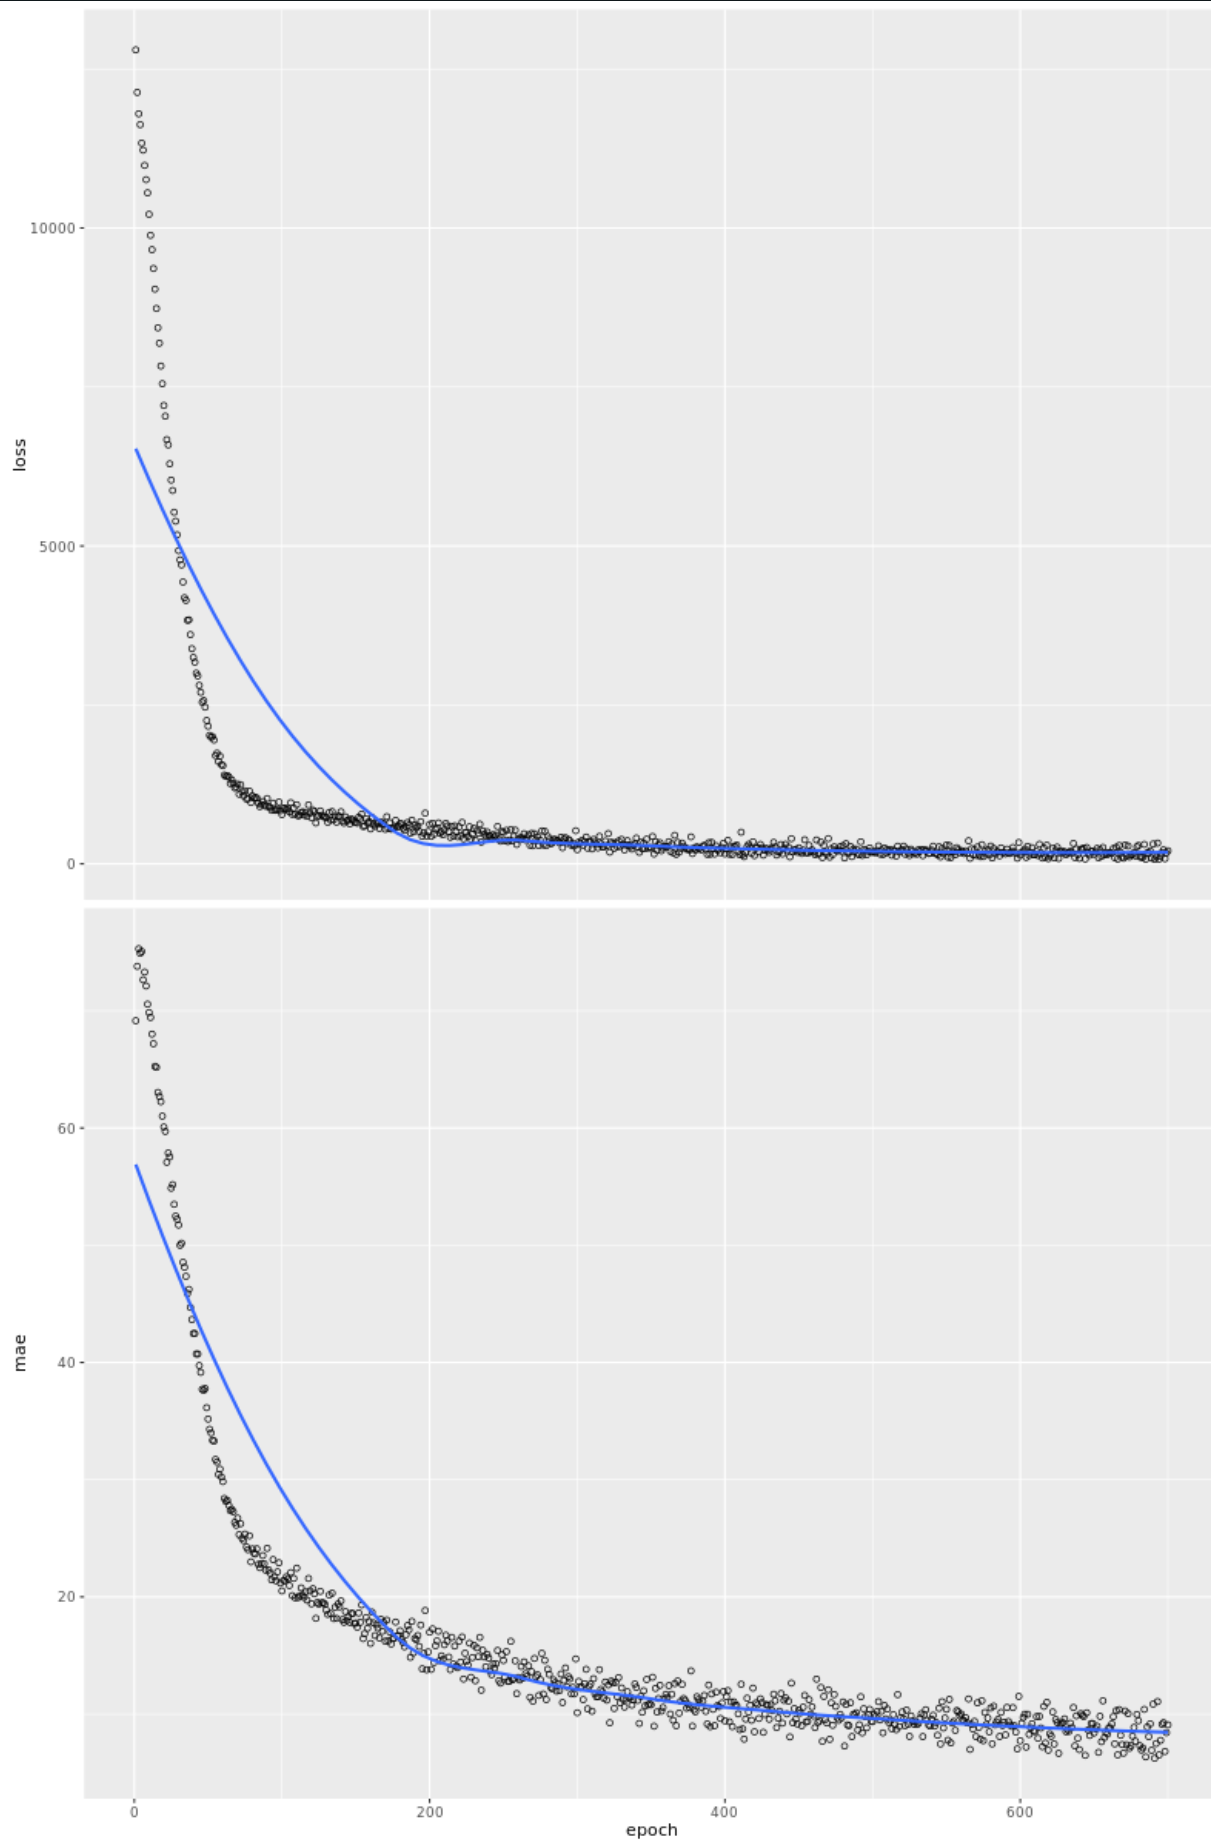
\includegraphics[width=7cm]{nn_loss}
		\caption{Loss (above) and MAE (below) of the Neural Network trained for Question 2.d}
		\label{fig:nn_loss}
	\end{figure}
	\begin{figure}[H]\centering
		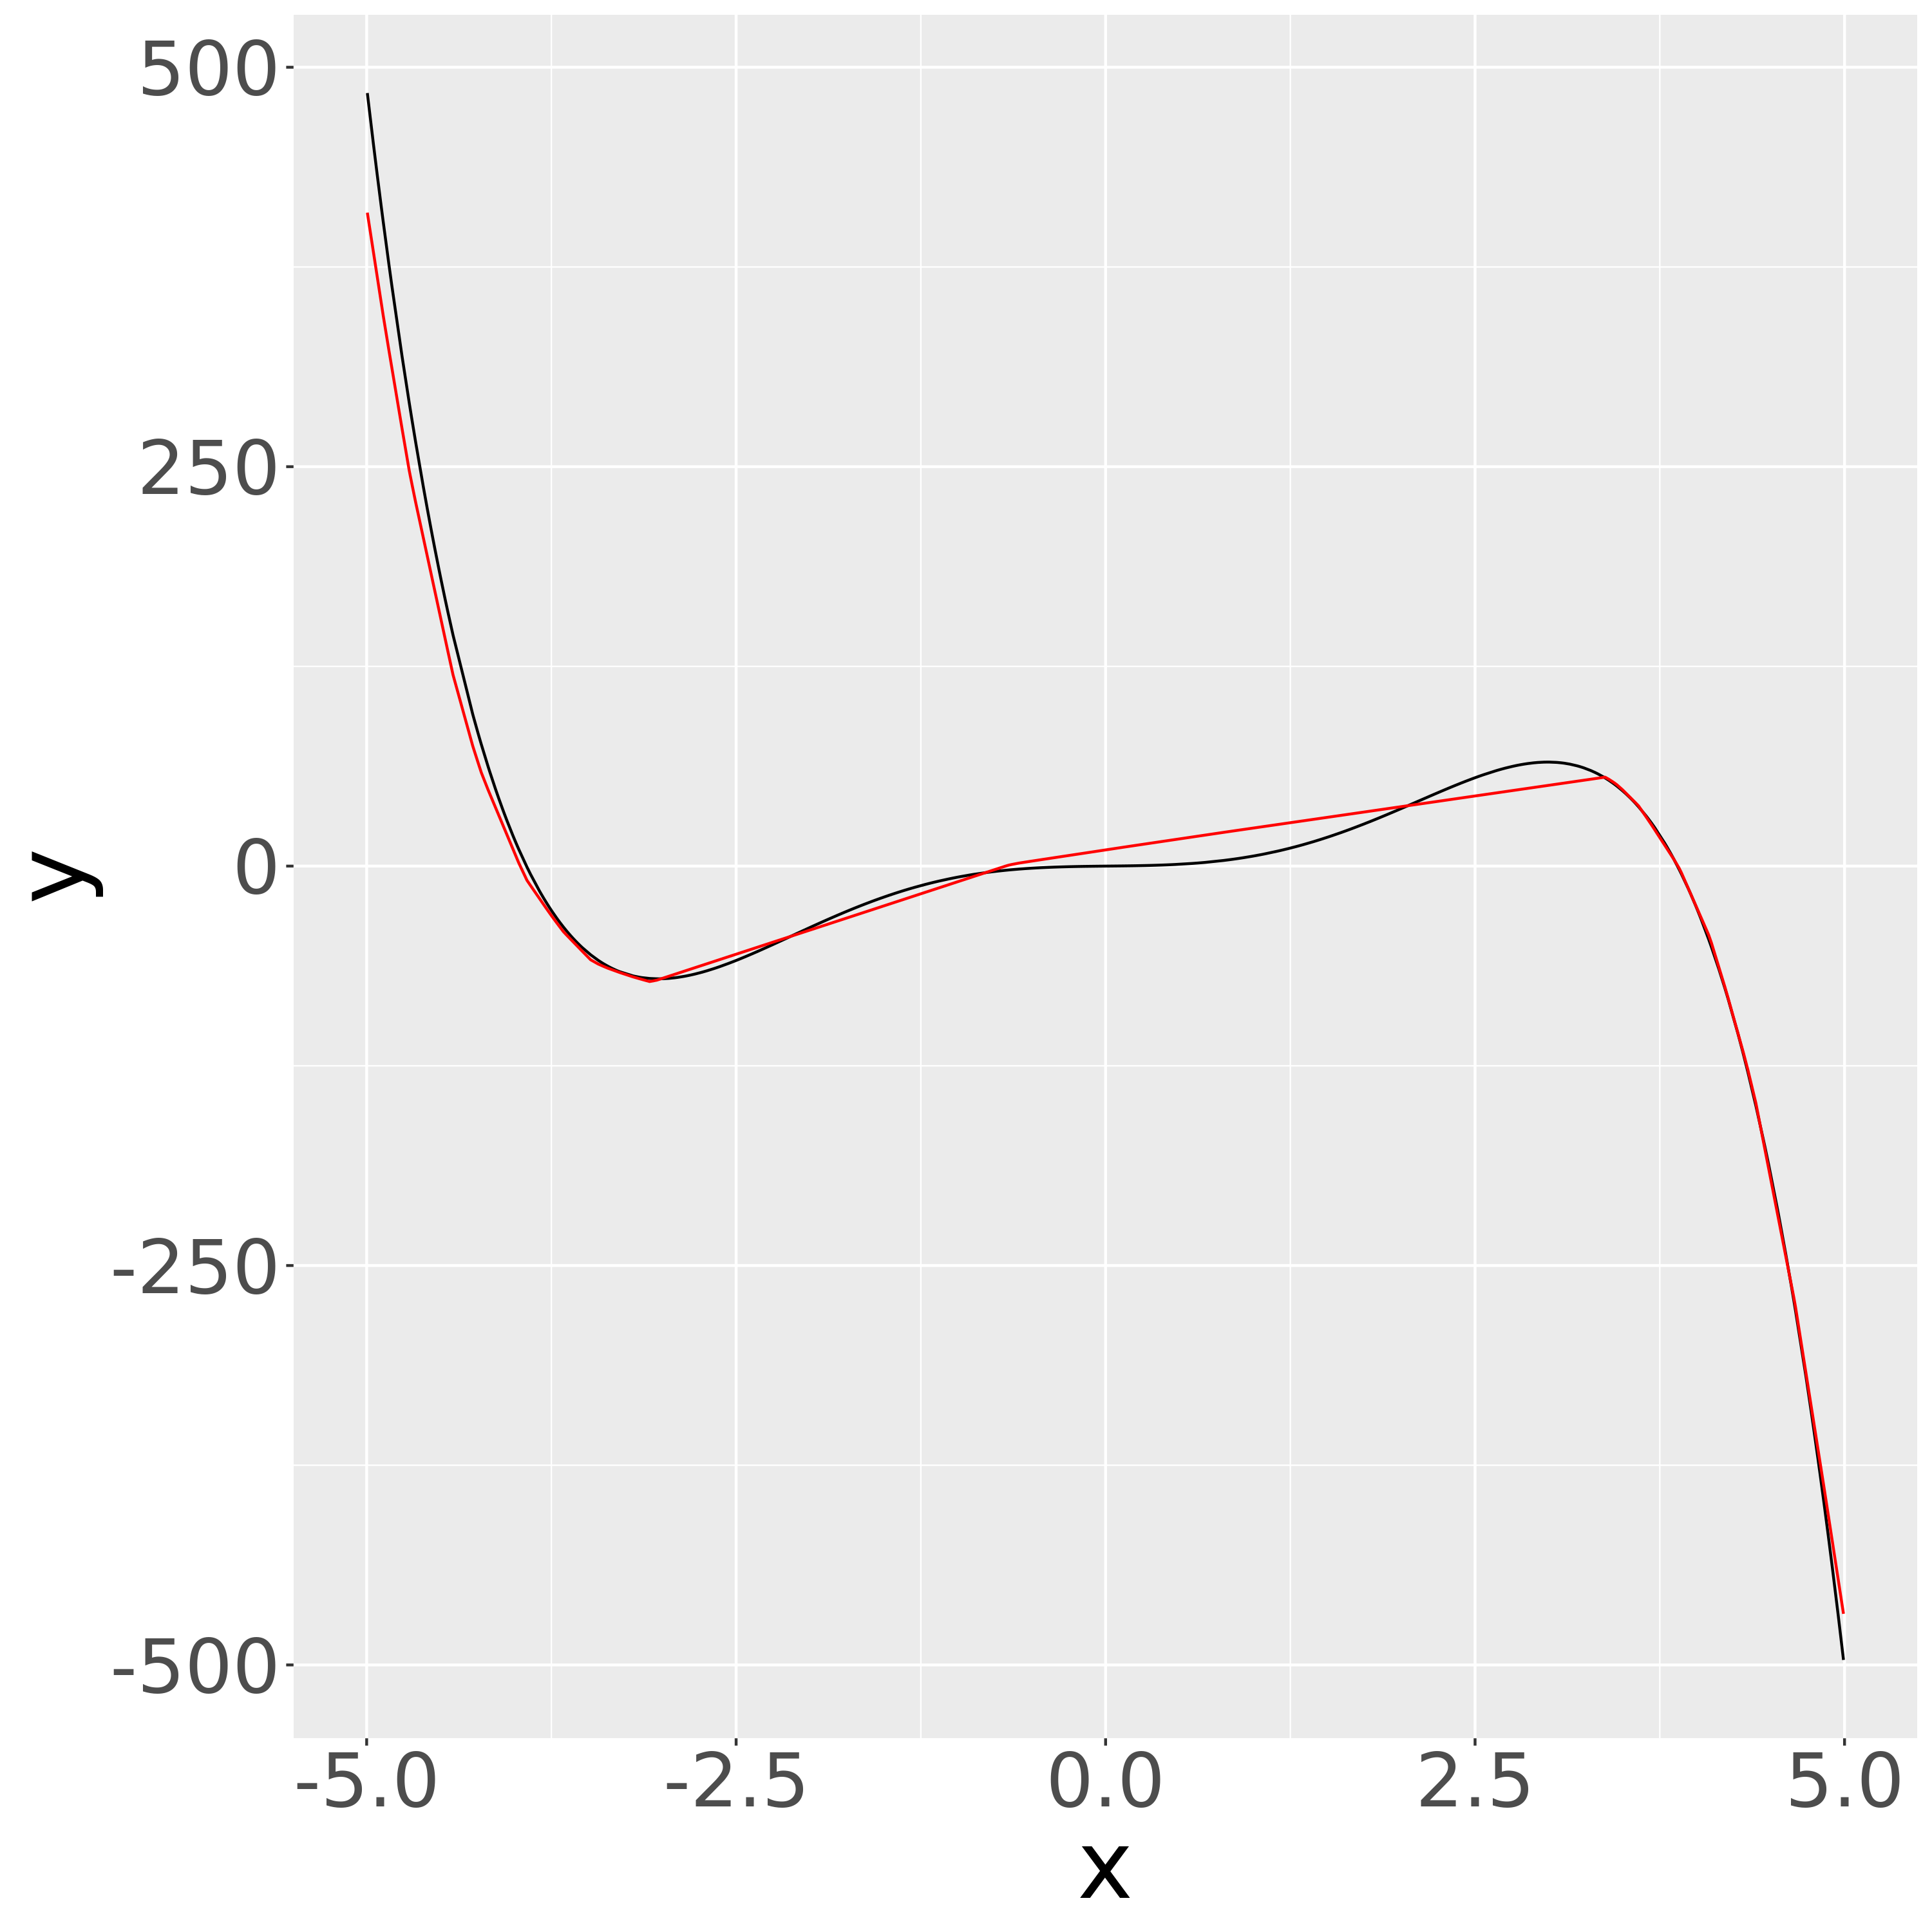
\includegraphics[width=7cm]{nn_preds}
		\caption{Comparison between the function fitted by the Neural Network (red) and the original function, or ground truth (black), from Question 2.d}
		\label{fig:nn_preds}
	\end{figure}
	
\end{enumerate}

\item Question 3

\begin{enumerate}
	\item Subquestion 3a 
	No missing values are present in any column.
	We know that the likelihood function is:
	\begin{equation}
		\operatorname{Pr}[\mathbf{X} \mid \boldsymbol{\beta}]=\prod_j \beta_j^{x_j}
	\end{equation}
	So the Lagrangian to maximize the likelihood is :
	\begin{equation}
		\mathfrak{L}(\boldsymbol{\beta}, \lambda)=\underbrace{\sum_j x_j \log \left(\beta_j\right)}_{\text {log-likelihood }}+\lambda \underbrace{\left(1-\sum_j \beta_j\right)}_{\text {Constraint on } \boldsymbol{\beta}}
	\end{equation}
	which can be solved by the MLE estimate $$\hat{\beta_j}= \frac{x_j}{N}$$, meanly the empirical frequency of the feature j
	So I computed the likelihood function as:
	\begin{equation}
		\operatorname{Pr}[\mathbf{X} \mid \boldsymbol{\beta}]=\prod_j \left(\frac{x_j}{N}\right)^{x_j}
	\end{equation}
	Unfortunately the likelihood value is too low to be stored in memory, because it is too closed to zero, so it is represented as zero.
	
	\item Subquestion 3b 
	When we assume heterogeneity across cells, we have to consider that the parameters $$\beta_{k,j}$$ are different for each category. Moreover, we model this heterogeneity as a cell-specific latent variable that can take one of K=2 values.
	So the likelihood function becomes:
	\begin{equation}
		\log\operatorname{Pr}[\mathbf{X} \mid \boldsymbol{\beta}]=\sum_{i}\log\sum_{k=1}^{2} \rho_k \prod_{j=1}^{220} \beta_{k,j}^{x_{i,j}}
	\end{equation}
	And we need to solve the optimization problem to find the parameters: $$\left[\rho_0^k,\beta_1^k,\beta_2^k,..,\beta_220^k\right]$$
	because number of categories=220. So we have $$(K-1)+K*(J-1)=(2-1)+2*(220-1)=439$$ parameters to estimate.
	\item Subquestion 3c 
	The following figures describe how the parameters differ across latent categories. Infact, based on the latent variable, they describe how likely is that the cell belongs to that category (like \textit{age\_group} or \textit{gender},..).
	\begin{figure}[H]\centering
		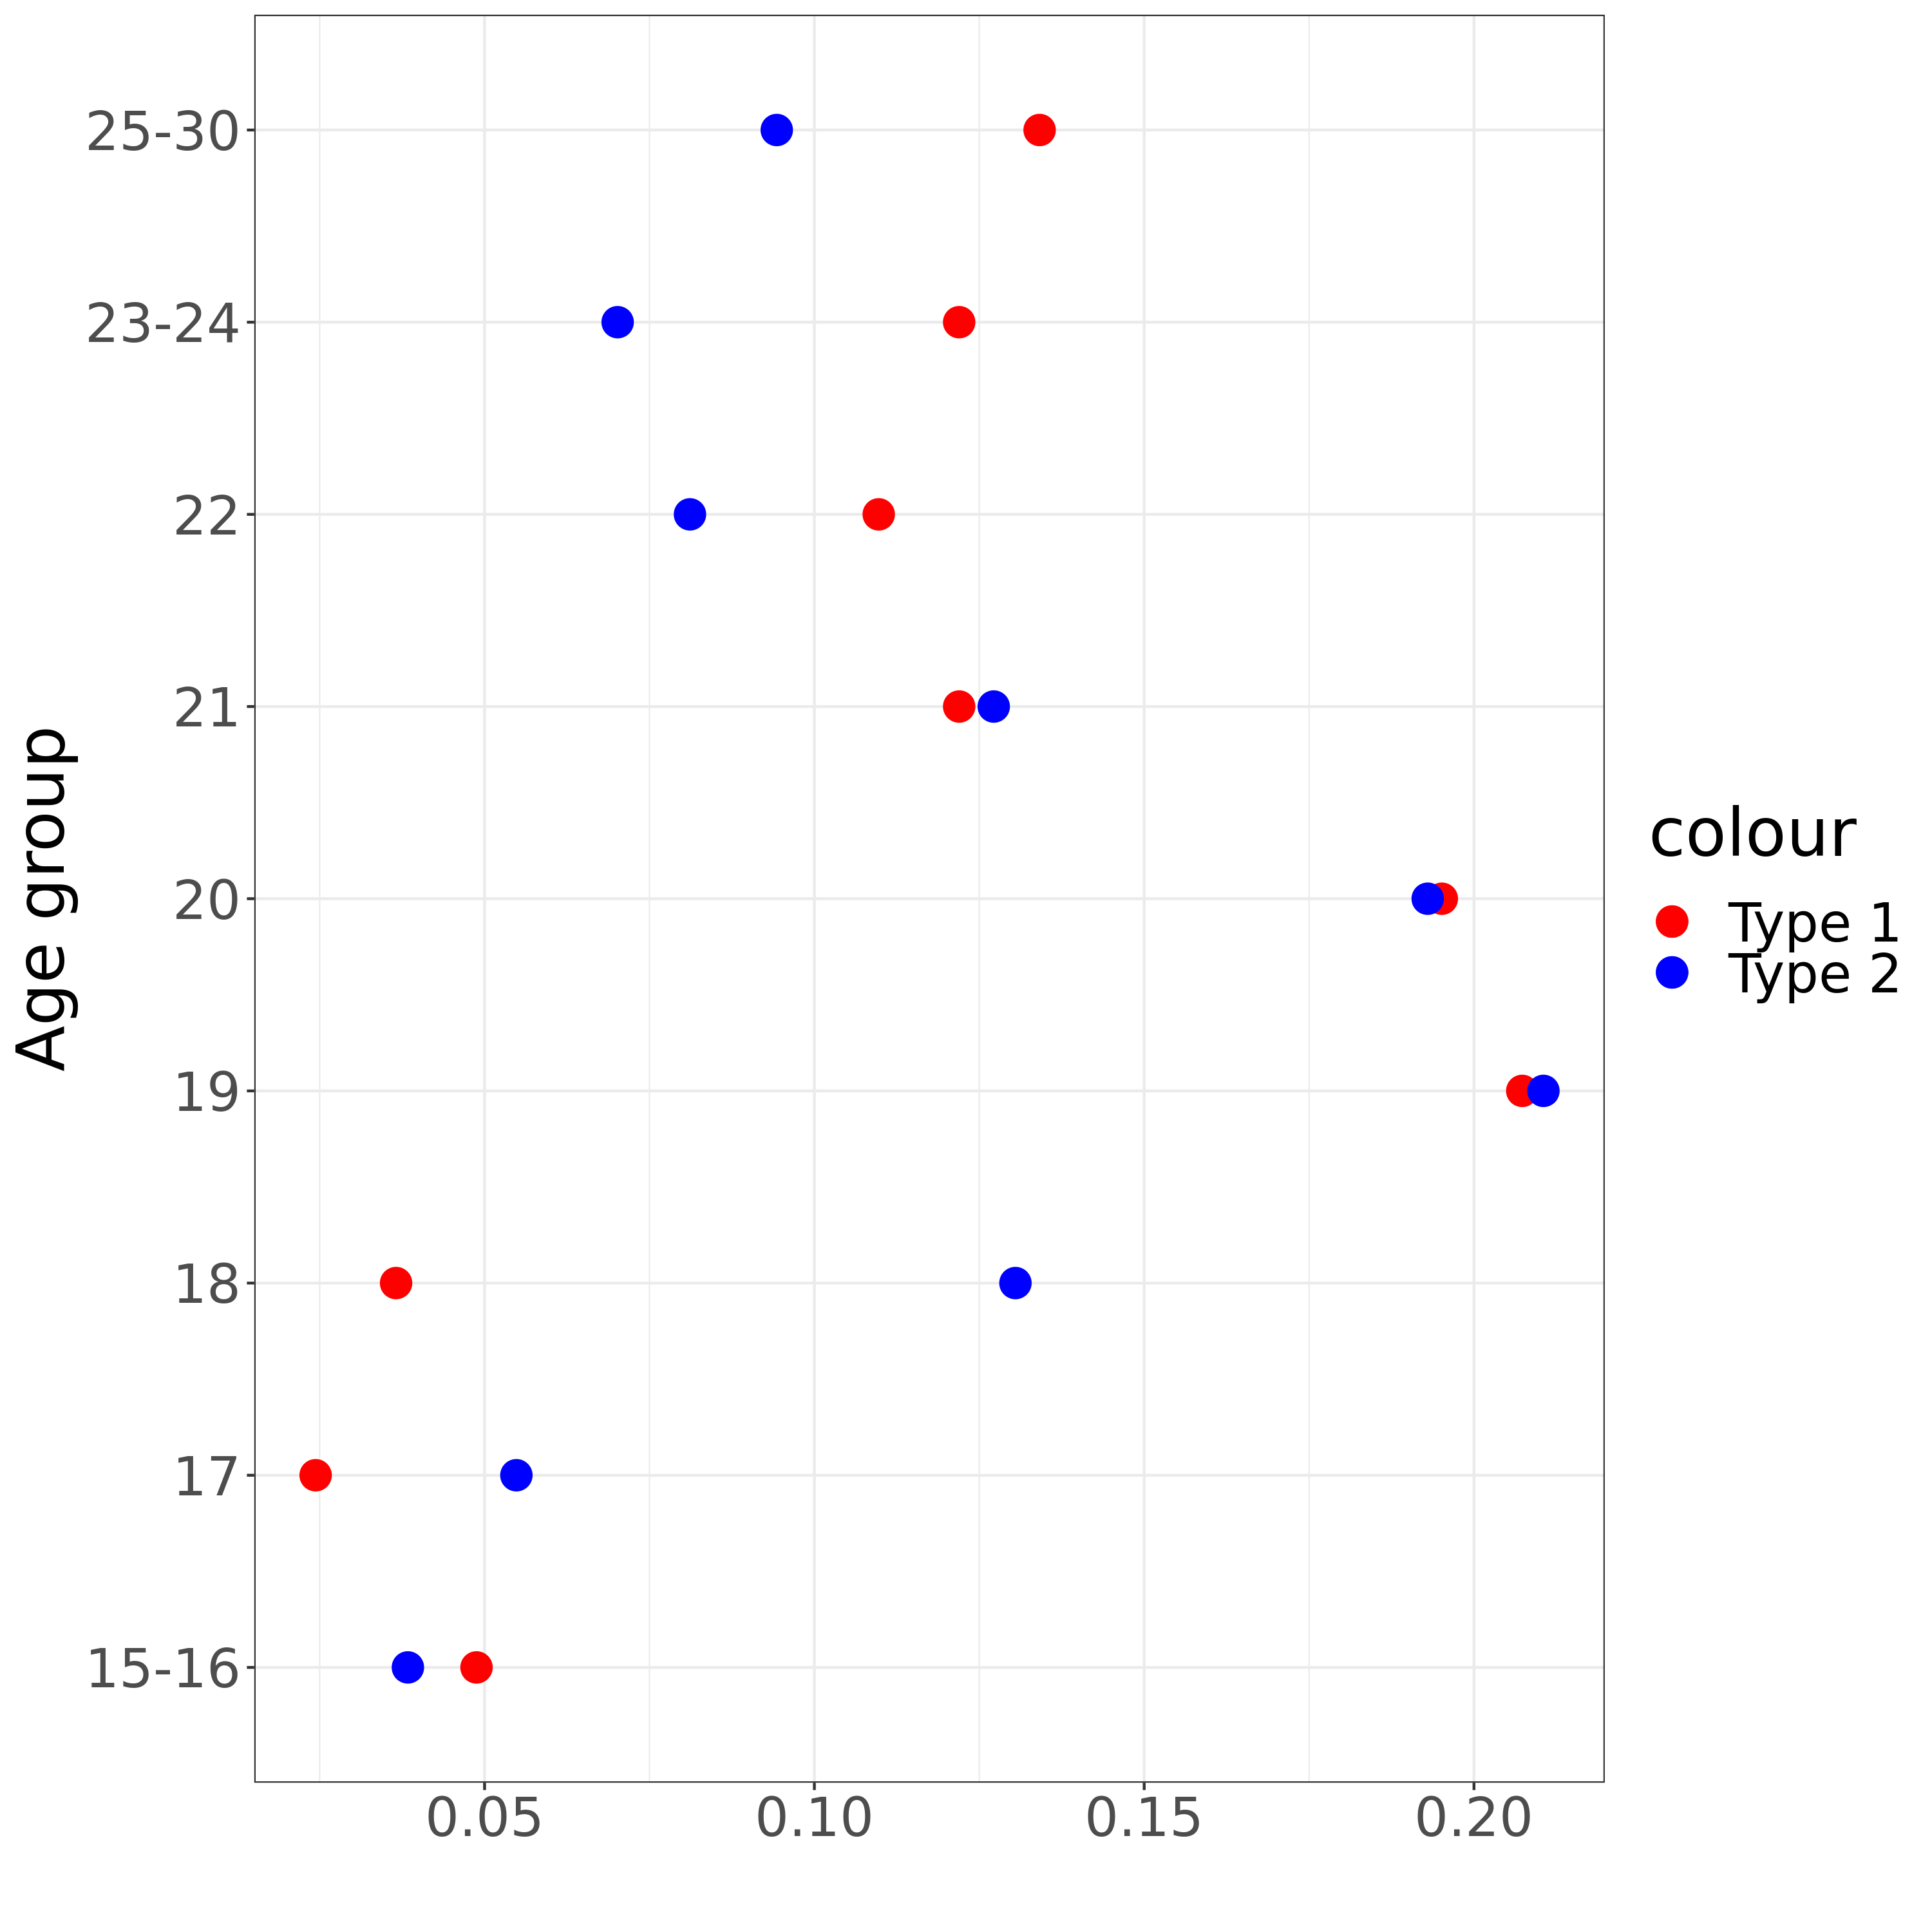
\includegraphics[width=7cm]{age_group}
		\caption{Comparison between the 2 types for each age\_group, from Question 3.c}
		\label{fig:age_group}
	\end{figure}
	\begin{figure}[H]\centering
		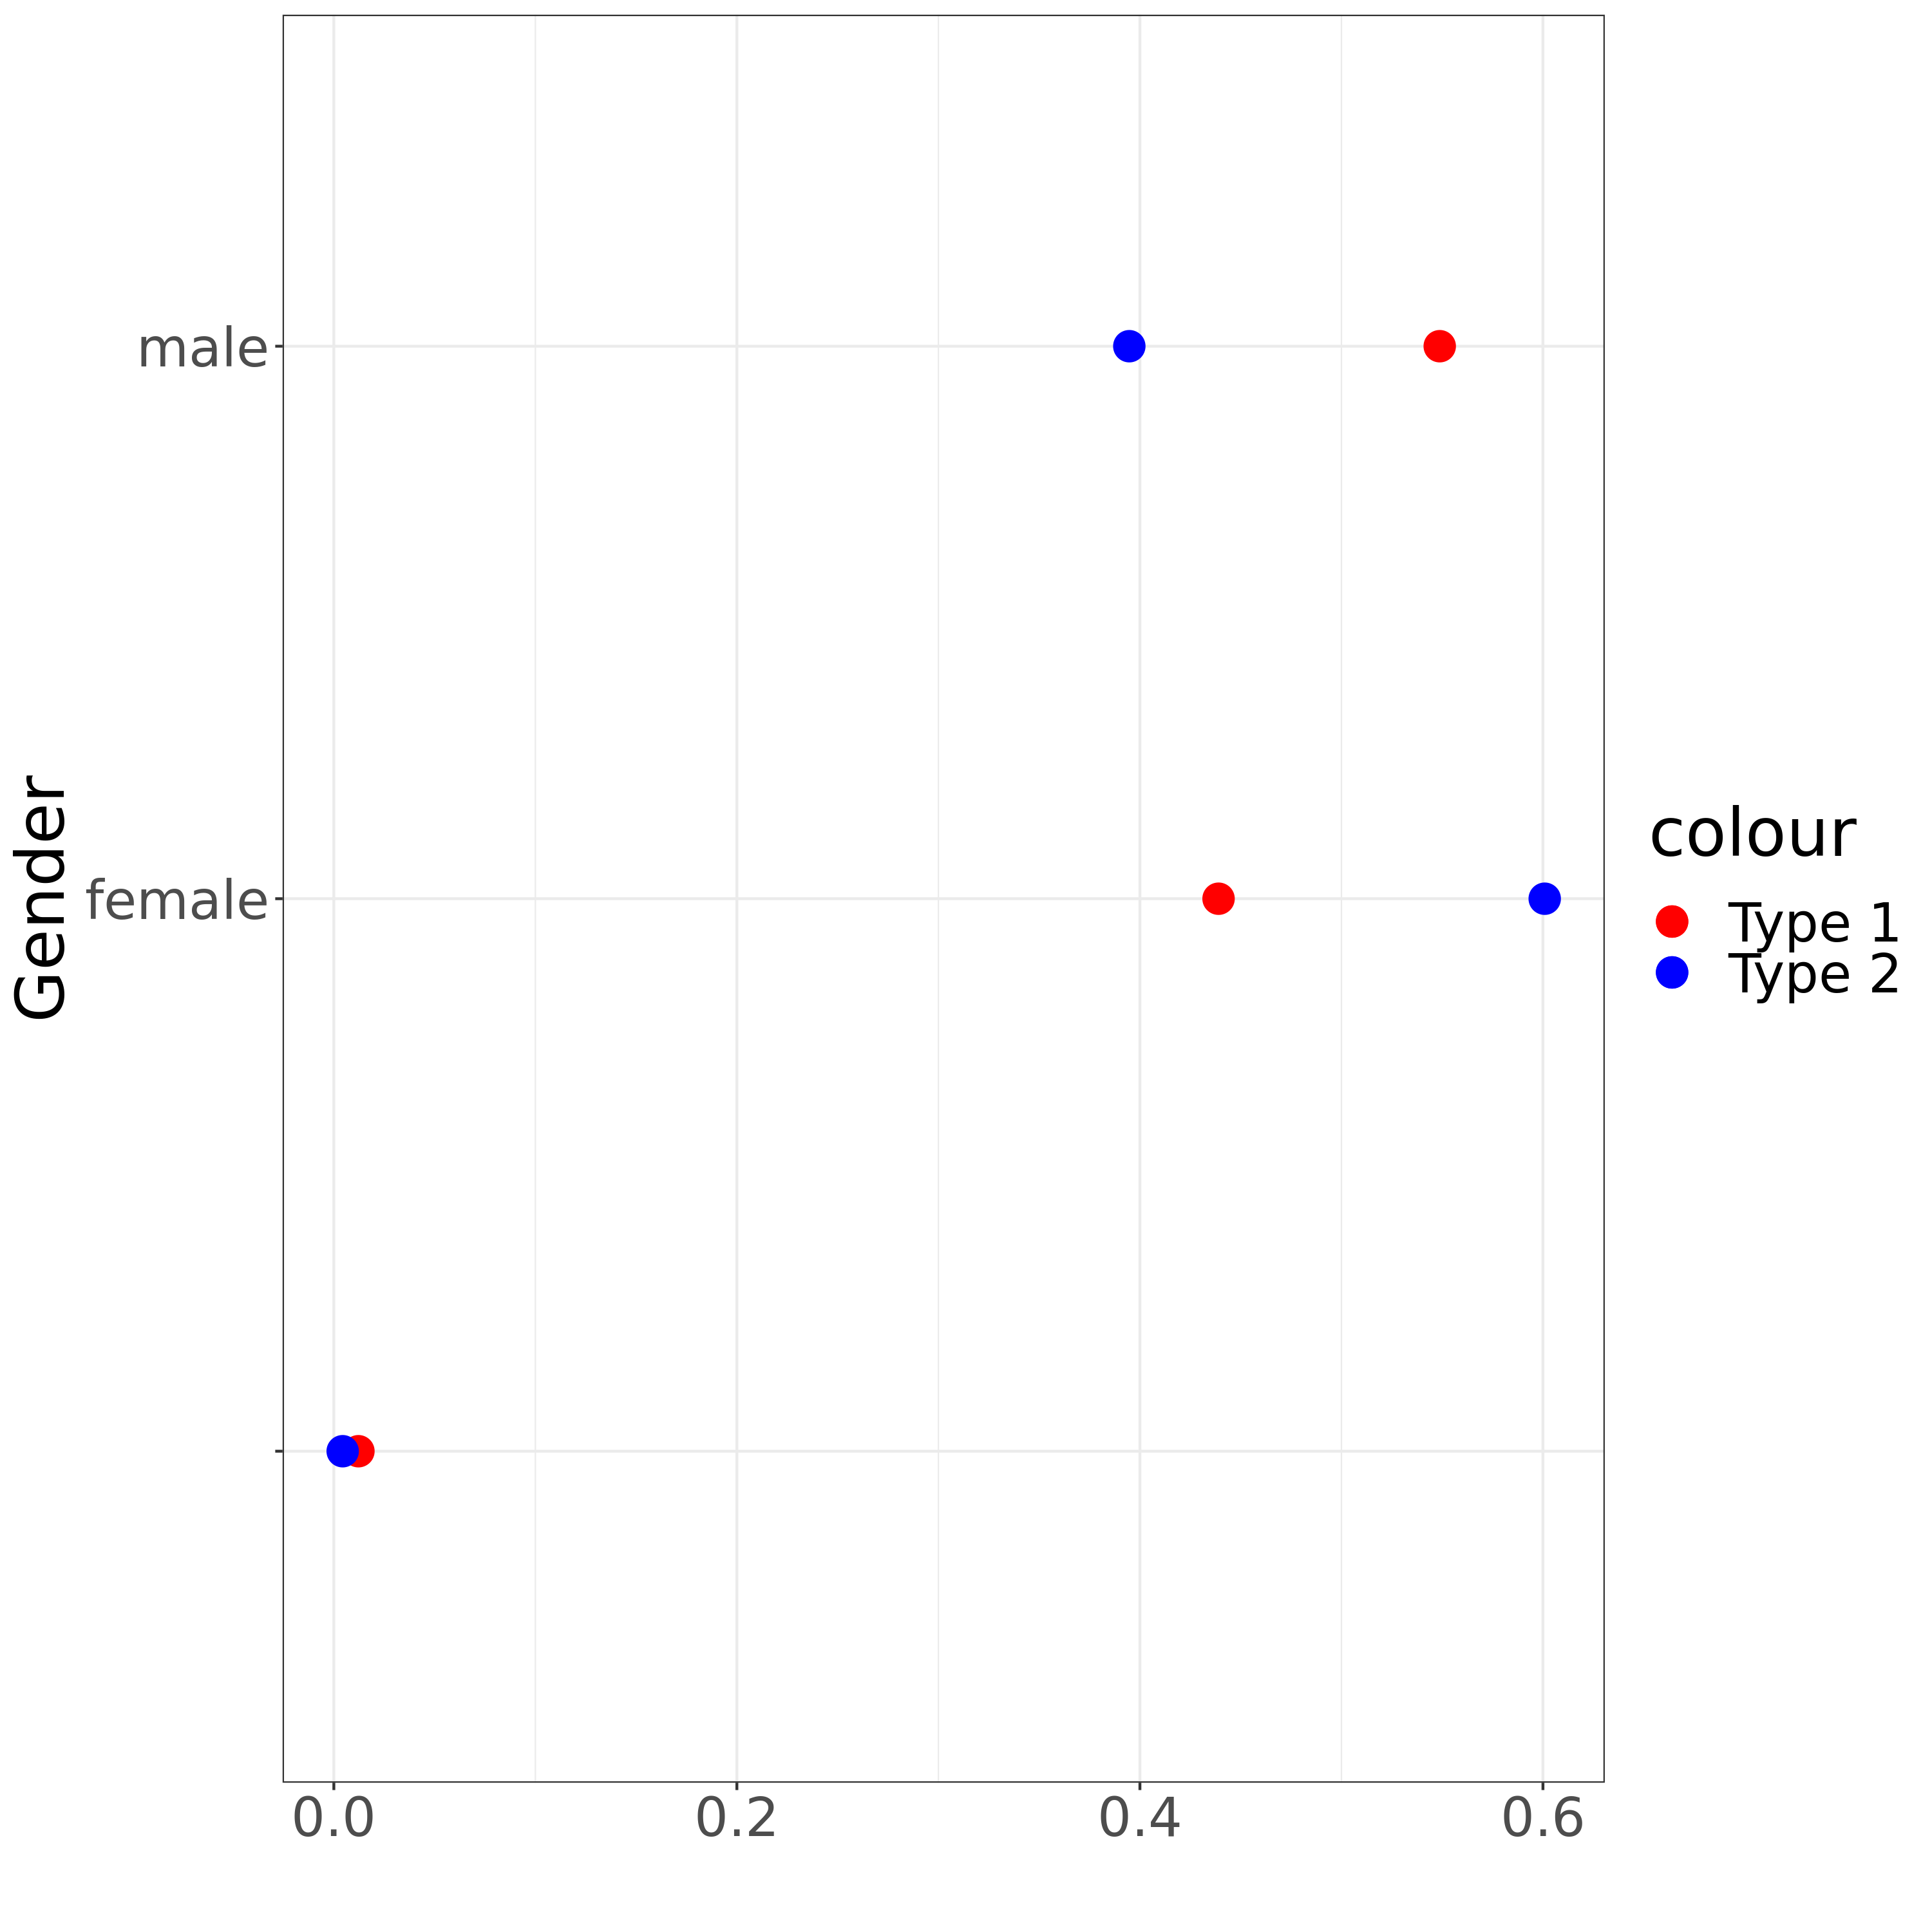
\includegraphics[width=7cm]{Gender}
		\caption{Comparison between the 2 types for each gender, from Question 3.c}
		\label{fig:age_group}
	\end{figure}
	\begin{figure}[H]\centering
		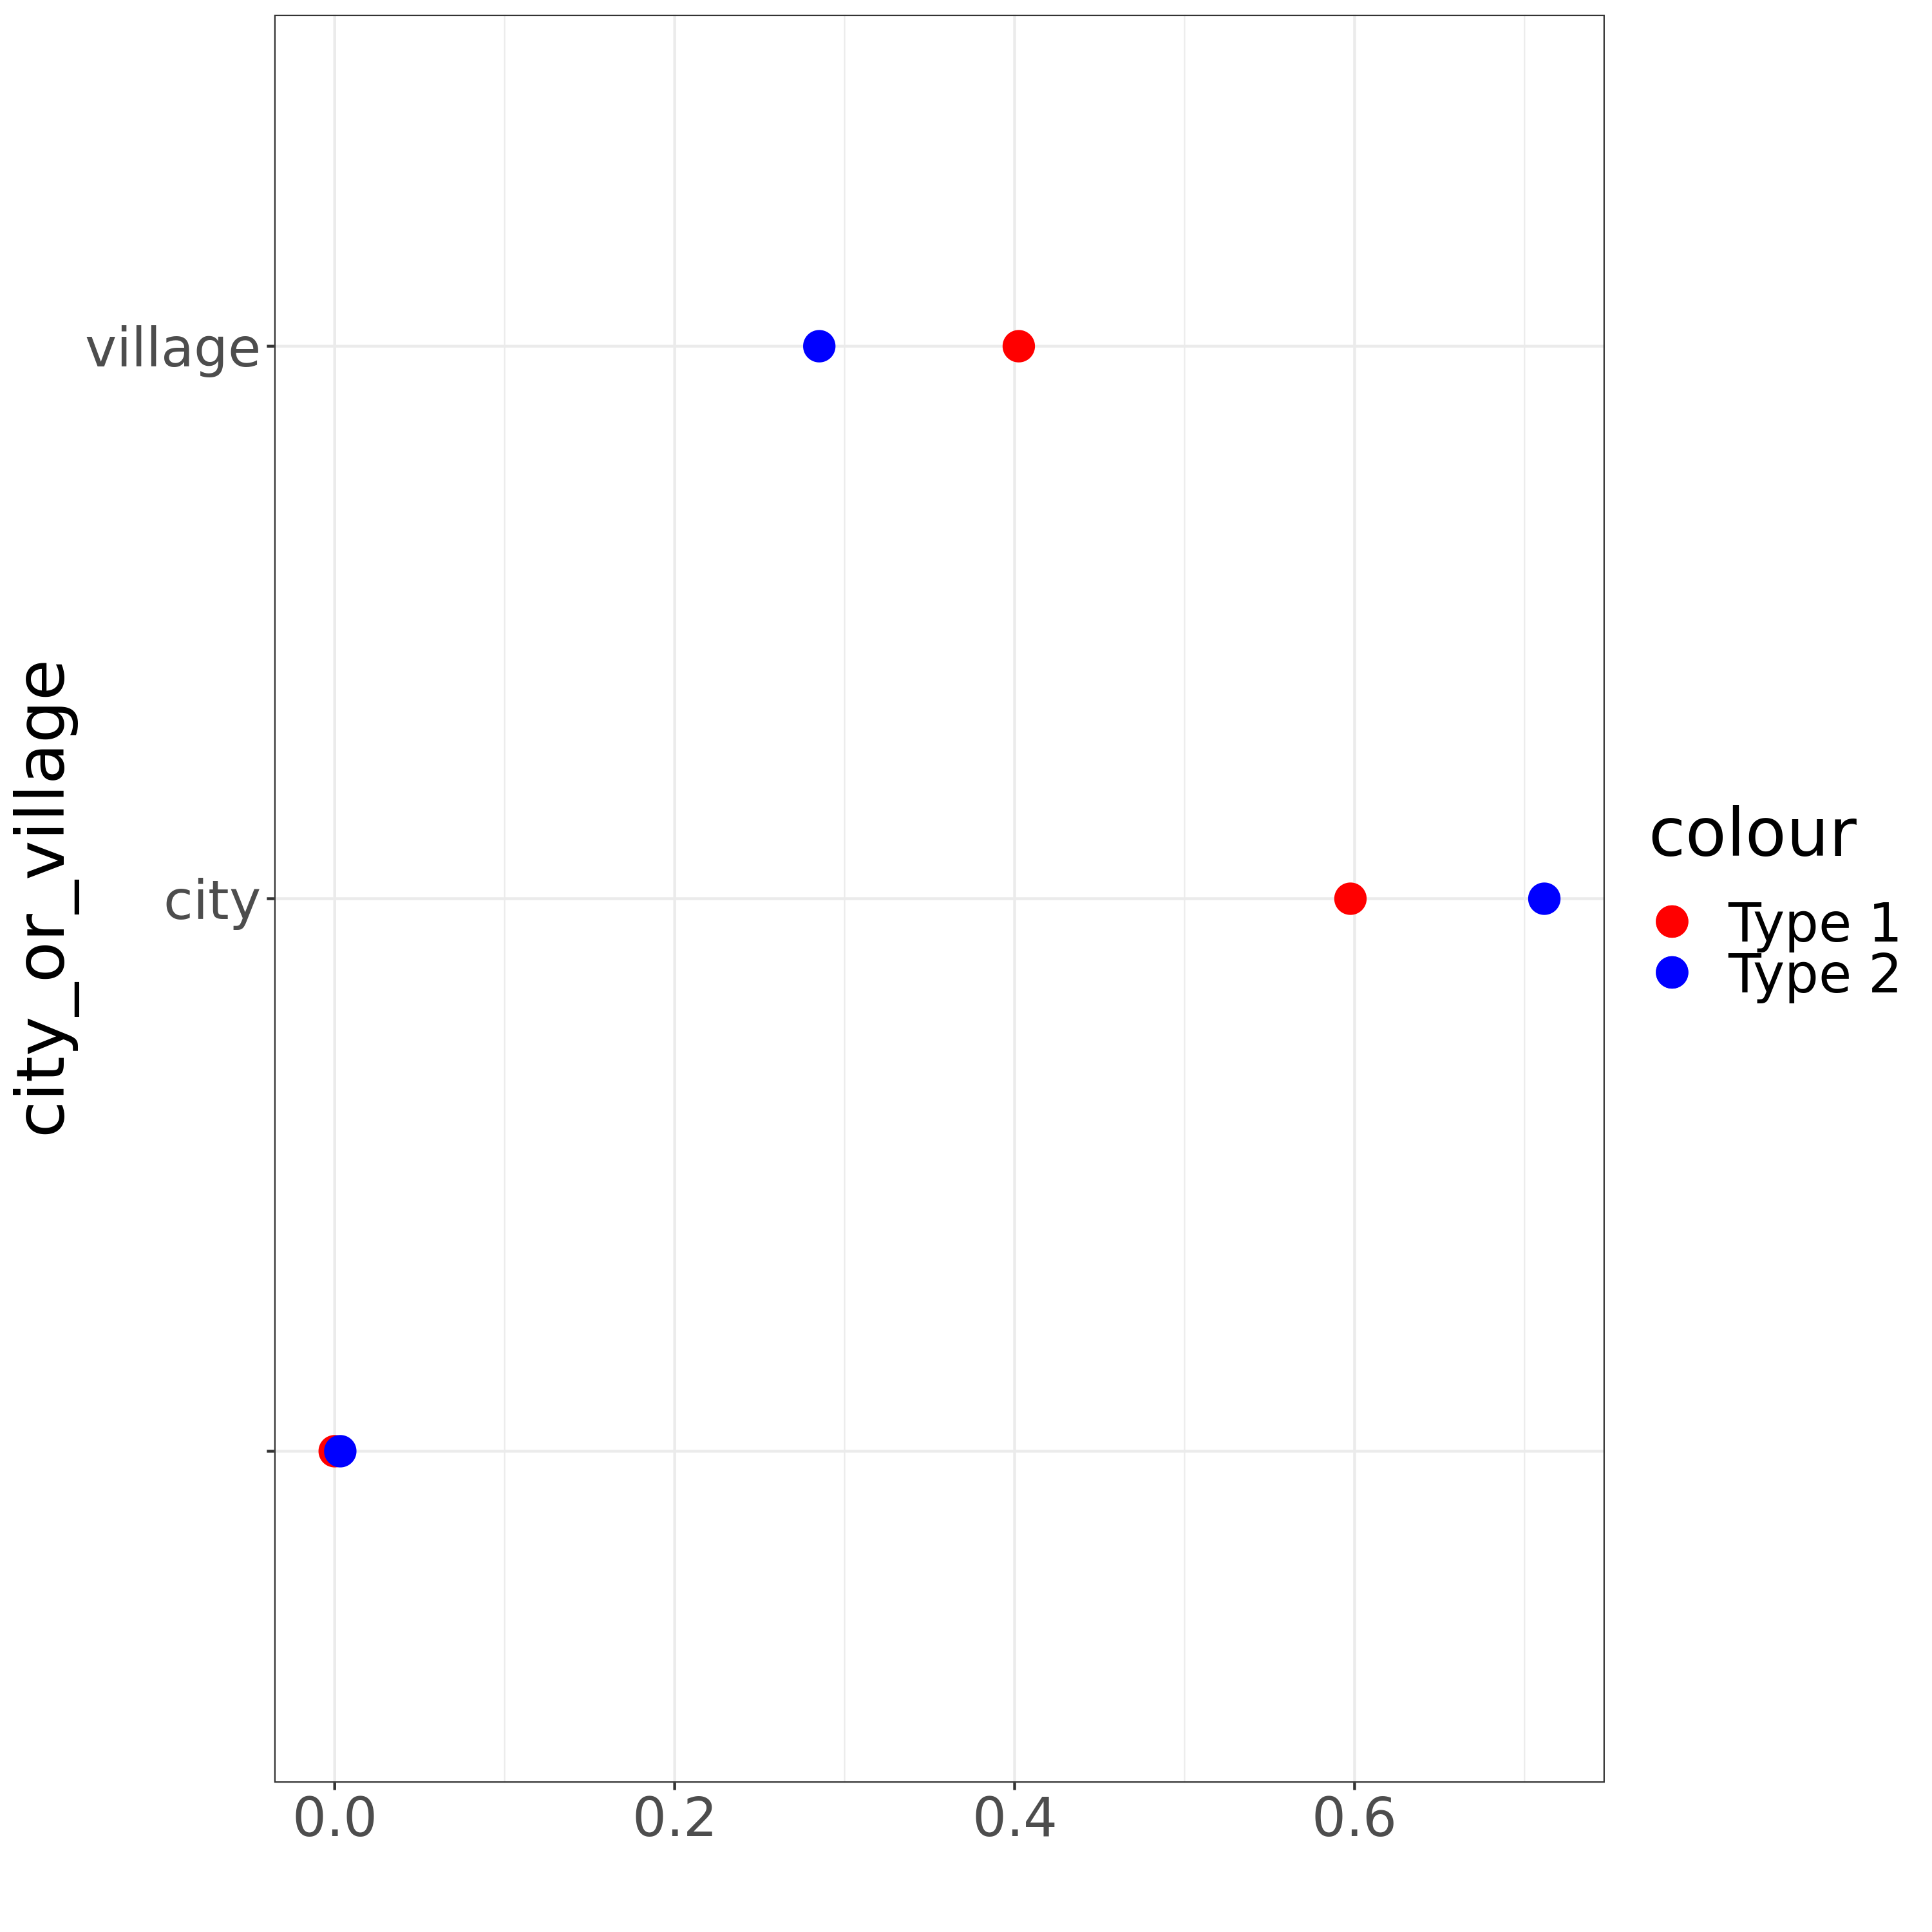
\includegraphics[width=7cm]{city_or_village}
		\caption{Comparison between the 2 types for the two groups from "city" or from "village", from Question 3.c}
		\label{fig:city_or_village}
	\end{figure}

	\item Subquestion 3d 

	\item Subquestion 3e here
\end{enumerate}

\end{enumerate}
\rfoot{END OF PAPER}

\end{document}
\grid
\grid
\grid
